%DIF 1c1
%DIF LATEXDIFF DIFFERENCE FILE
%DIF DEL main.tex            Wed Mar  6 16:12:09 2024
%DIF ADD main-revision.tex   Wed Mar  6 16:12:09 2024
%DIF < %! BibTeX Compiler = biber
%DIF -------
%! BibTeX Compiler = bibtex %DIF > 
%DIF -------
%TC:ignore
\documentclass{article}
\usepackage{caption}
\usepackage{censor}
\usepackage{xcolor, colortbl}
\definecolor{BLUELINK}{HTML}{0645AD}
\definecolor{DARKBLUELINK}{HTML}{0B0080}
\definecolor{LIGHTGREY}{gray}{0.9}
\PassOptionsToPackage{hyphens}{url}
\usepackage[colorlinks=false]{hyperref}
% for linking between references, figures, TOC, etc in the pdf document
\hypersetup{colorlinks,
    linkcolor=DARKBLUELINK,
    anchorcolor=DARKBLUELINK,
    citecolor=DARKBLUELINK,
    filecolor=DARKBLUELINK,
    menucolor=DARKBLUELINK,
    urlcolor=BLUELINK
} % Color citation links in purple
\PassOptionsToPackage{unicode}{hyperref}
\PassOptionsToPackage{naturalnames}{hyperref}

\usepackage{biorxiv}

\usepackage{url}
\usepackage{amssymb,amsfonts,amsmath,amsthm,mathtools}
\usepackage{lmodern}
\usepackage{xfrac, nicefrac}
\usepackage{bm}
\usepackage{listings, enumerate, enumitem}
\usepackage[export]{adjustbox}
\usepackage{graphicx}
\usepackage{bbold}
\usepackage{pdfpages}
\pdfinclusioncopyfonts=1
\usepackage{lineno}
\usepackage{tabu}
\usepackage{hhline}
\usepackage{multicol,multirow,array}
\usepackage{etoolbox}
\usepackage{booktabs}
\usepackage{makecell}
%DIF 44d44
%DIF < \usepackage{orcidlink}
%DIF -------
\usepackage{marvosym}

% -- Defining colors:
\definecolor{backcolour}{rgb}{0.95,0.95,0.92}% Definig a custom style:
\lstdefinestyle{mystyle}{
    backgroundcolor=\color{backcolour},
    basicstyle=\ttfamily\scriptsize\bfseries,
    breakatwhitespace=false,
    breaklines=true,
    captionpos=t,
    keepspaces=true,
    showspaces=false,
    showstringspaces=false,
    showtabs=false,
    tabsize=2
}% -- Setting up the custom style:
\lstset{style=mystyle}
\captionsetup[table]{hypcap=false}
\captionsetup[figure]{hypcap=false}

\newcommand{\defEqual}{\stackrel{\text{def}}{=}}
\newcommand{\Multiply}{\cdot}
\newcommand{\MultiplyMatrix}{\times}
\newcommand{\UniDimArray}[1]{\bm{#1}}
\newcommand{\BiDimArray}[1]{\bm{#1}}
\newcommand{\tr}{^{\intercal}}
\newcommand{\inv}{^{-1}}
\DeclareMathOperator{\E}{\mathbb{E}}
%DIF 73-74c72-73
%DIF < \DeclareMathOperator{\Var}{\text{Var}}
%DIF < \DeclareMathOperator{\Cov}{\text{Cov}}
%DIF -------
\DeclareMathOperator{\Var}{\text{var}} %DIF > 
\DeclareMathOperator{\Cov}{\text{cov}} %DIF > 
%DIF -------
\newcommand{\Qst}{Q$_\text{ST}$}
\newcommand{\Fst}{F$_\text{ST}$}
\newcommand{\QstFst}{\Qst--\Fst}
\newcommand{\der}{\mathrm{d}}
\newcommand{\e}{\text{e}}
\newcommand{\Ne}{N_{\text{e}}}
\newcommand{\dnds}{\omega}
\newcommand{\pn}{\pi_N}
\newcommand{\ps}{\pi_S}
\newcommand{\pnps}{\pn / \ps}
\newcommand{\proba}{\mathbb{P}}
\newcommand{\pfix}{\proba_{\text{fix}}}
\newcommand{\Spi}{i}
\newcommand{\Spj}{j}
\newcommand{\NbrTaxa}{n}
%DIF 90c89-92
%DIF < \newcommand{\Time}{t}
%DIF -------
\newcommand{\Time}{T} %DIF > 
\newcommand{\GenTime}{\tau} %DIF > 
\newcommand{\NbrGen}{t_{\Spi, \Spj}} %DIF > 
\newcommand{\NucDiv}{d_{\Spi, \Spj}} %DIF > 
%DIF -------
\newcommand{\Trait}{P}
\newcommand{\Heritability}{h^2}
\newcommand{\HeritabilitySpi}{\Heritability_{\Spi}}
%DIF 94c96
%DIF < \newcommand{\MeanTrait}{\bar{\Trait_{\Time}}}
%DIF -------
\newcommand{\MeanTrait}{\bar{\Trait}} %DIF > 
%DIF -------
\newcommand{\VecTrait}{\UniDimArray{\bar{\Trait}}}
%DIF 96-98c98-99
%DIF < \newcommand{\Root}{0}
%DIF < \newcommand{\RootTrait}{\Trait_{\Root}}
%DIF < \newcommand{\VarPhy}{\Var \left[\MeanTrait\right]}
%DIF -------
\newcommand{\RootTrait}{\theta} %DIF > 
\newcommand{\VarPhy}{\Cov \left( \MeanTrait_{\Spi}, \MeanTrait_{\Spj}\right)} %DIF > 
%DIF -------
\newcommand{\VecZero}{\UniDimArray{0}}
\newcommand{\VecOne}{\UniDimArray{1}}
\newcommand{\Distance}{\BiDimArray{D}}
\newcommand{\DistanceMatrix}{\BiDimArray{\Distance}}
\newcommand{\MutationRatePheno}{\mu}
%DIF 104a105
\newcommand{\MutationRateNuc}{u} %DIF > 
%DIF -------
\newcommand{\SubRate}{q}
\newcommand{\NbrLoci}{L}
\newcommand{\VarPhenotype}{V_{\Trait}}
\newcommand{\VarPhenotypeSpi}{V_{\Trait, \Spi}}
\newcommand{\VarGenetic}{V_{\mathrm{A}}}
\newcommand{\VarGeneticSpi}{V_{\mathrm{A}, \Spi}}
\newcommand{\VarEnv}{V_{\mathrm{E}}}
\newcommand{\VarMutation}{V_{\mathrm{M}}}
\newcommand{\GenArchi}{\NbrLoci \Multiply \E \left[ a^2 \right]}
\newcommand{\RateMut}{\sigma^2_{\mathrm{M}}}
\newcommand{\RateBetween}{\sigma^2_{\mathrm{B}}}
\newcommand{\RateWhithin}{\sigma^2_{\mathrm{W}}}
\newcommand{\RateWhithinSpi}{\sigma^2_{\mathrm{W}, \Spi}}
\newcommand{\VecRateWhithin}{\UniDimArray{\RateWhithin}}
\newcommand{\EstRateBetween}{\widehat{\RateBetween}}
\newcommand{\EstRateWhithin}{\widehat{\RateWhithin}}
\newcommand{\NI}{\rho}
\newcommand{\EstNI}{\widehat{\rho}}
\newcommand{\StdSelection}{\sigma}
\newcommand{\VarSelection}{\StdSelection^2}

% Tree
\newcommand{\Nbranch}{2 \NbrTaxa - 2}
\newcommand{\WishartPostDf}{2 \NbrTaxa + 1}
\newcommand{\Ntrait}{K}
\newcommand{\contrast}{\UniDimArray{C}}
\newcommand{\Covariancematrix}{\Sigma}
\newcommand{\CovarianceMatrix}{\BiDimArray{\Covariancematrix}}
\newcommand{\Precisionmatrix}{\Omega}
\newcommand{\PrecisionMatrix}{\BiDimArray{\Precisionmatrix}}
\newcommand{\Identitymatrix}{\BiDimArray{I}}
\newcommand{\brownian}{\mathcal{B}}
\newcommand{\Brownian}{\UniDimArray{\brownian}}
\newcommand{\Scattermatrix}{\BiDimArray{A}}
\newcommand{\Multivariate}{\UniDimArray{Z}}

\renewcommand{\baselinestretch}{1.5}
\renewcommand{\arraystretch}{1.2}
\linenumbers
\frenchspacing

\title{Detecting diversifying selection for a trait from within and between-species genotypes and phenotypes}
\rhead{\scshape Trait selection from within and between-species variation}

\author{~}
%DIF PREAMBLE EXTENSION ADDED BY LATEXDIFF
%DIF UNDERLINE PREAMBLE %DIF PREAMBLE
\RequirePackage[normalem]{ulem} %DIF PREAMBLE
\RequirePackage{color}\definecolor{RED}{rgb}{1,0,0}\definecolor{BLUE}{rgb}{0,0,1} %DIF PREAMBLE
\providecommand{\DIFaddtex}[1]{{\protect\color{blue}\uwave{#1}}} %DIF PREAMBLE
\providecommand{\DIFdeltex}[1]{{\protect\color{red}\sout{#1}}}                      %DIF PREAMBLE
%DIF SAFE PREAMBLE %DIF PREAMBLE
\providecommand{\DIFaddbegin}{} %DIF PREAMBLE
\providecommand{\DIFaddend}{} %DIF PREAMBLE
\providecommand{\DIFdelbegin}{} %DIF PREAMBLE
\providecommand{\DIFdelend}{} %DIF PREAMBLE
\providecommand{\DIFmodbegin}{} %DIF PREAMBLE
\providecommand{\DIFmodend}{} %DIF PREAMBLE
%DIF FLOATSAFE PREAMBLE %DIF PREAMBLE
\providecommand{\DIFaddFL}[1]{\DIFadd{#1}} %DIF PREAMBLE
\providecommand{\DIFdelFL}[1]{\DIFdel{#1}} %DIF PREAMBLE
\providecommand{\DIFaddbeginFL}{} %DIF PREAMBLE
\providecommand{\DIFaddendFL}{} %DIF PREAMBLE
\providecommand{\DIFdelbeginFL}{} %DIF PREAMBLE
\providecommand{\DIFdelendFL}{} %DIF PREAMBLE
%DIF HYPERREF PREAMBLE %DIF PREAMBLE
\providecommand{\DIFadd}[1]{\texorpdfstring{\DIFaddtex{#1}}{#1}} %DIF PREAMBLE
\providecommand{\DIFdel}[1]{\texorpdfstring{\DIFdeltex{#1}}{}} %DIF PREAMBLE
\newcommand{\DIFscaledelfig}{0.5}
%DIF HIGHLIGHTGRAPHICS PREAMBLE %DIF PREAMBLE
\RequirePackage{settobox} %DIF PREAMBLE
\RequirePackage{letltxmacro} %DIF PREAMBLE
\newsavebox{\DIFdelgraphicsbox} %DIF PREAMBLE
\newlength{\DIFdelgraphicswidth} %DIF PREAMBLE
\newlength{\DIFdelgraphicsheight} %DIF PREAMBLE
% store original definition of \includegraphics %DIF PREAMBLE
\LetLtxMacro{\DIFOincludegraphics}{\includegraphics} %DIF PREAMBLE
\newcommand{\DIFaddincludegraphics}[2][]{{\color{blue}\fbox{\DIFOincludegraphics[#1]{#2}}}} %DIF PREAMBLE
\newcommand{\DIFdelincludegraphics}[2][]{% %DIF PREAMBLE
\sbox{\DIFdelgraphicsbox}{\DIFOincludegraphics[#1]{#2}}% %DIF PREAMBLE
\settoboxwidth{\DIFdelgraphicswidth}{\DIFdelgraphicsbox} %DIF PREAMBLE
\settoboxtotalheight{\DIFdelgraphicsheight}{\DIFdelgraphicsbox} %DIF PREAMBLE
\scalebox{\DIFscaledelfig}{% %DIF PREAMBLE
\parbox[b]{\DIFdelgraphicswidth}{\usebox{\DIFdelgraphicsbox}\\[-\baselineskip] \rule{\DIFdelgraphicswidth}{0em}}\llap{\resizebox{\DIFdelgraphicswidth}{\DIFdelgraphicsheight}{% %DIF PREAMBLE
\setlength{\unitlength}{\DIFdelgraphicswidth}% %DIF PREAMBLE
\begin{picture}(1,1)% %DIF PREAMBLE
\thicklines\linethickness{2pt} %DIF PREAMBLE
{\color[rgb]{1,0,0}\put(0,0){\framebox(1,1){}}}% %DIF PREAMBLE
{\color[rgb]{1,0,0}\put(0,0){\line( 1,1){1}}}% %DIF PREAMBLE
{\color[rgb]{1,0,0}\put(0,1){\line(1,-1){1}}}% %DIF PREAMBLE
\end{picture}% %DIF PREAMBLE
}\hspace*{3pt}}} %DIF PREAMBLE
} %DIF PREAMBLE
\LetLtxMacro{\DIFOaddbegin}{\DIFaddbegin} %DIF PREAMBLE
\LetLtxMacro{\DIFOaddend}{\DIFaddend} %DIF PREAMBLE
\LetLtxMacro{\DIFOdelbegin}{\DIFdelbegin} %DIF PREAMBLE
\LetLtxMacro{\DIFOdelend}{\DIFdelend} %DIF PREAMBLE
\DeclareRobustCommand{\DIFaddbegin}{\DIFOaddbegin \let\includegraphics\DIFaddincludegraphics} %DIF PREAMBLE
\DeclareRobustCommand{\DIFaddend}{\DIFOaddend \let\includegraphics\DIFOincludegraphics} %DIF PREAMBLE
\DeclareRobustCommand{\DIFdelbegin}{\DIFOdelbegin \let\includegraphics\DIFdelincludegraphics} %DIF PREAMBLE
\DeclareRobustCommand{\DIFdelend}{\DIFOaddend \let\includegraphics\DIFOincludegraphics} %DIF PREAMBLE
\LetLtxMacro{\DIFOaddbeginFL}{\DIFaddbeginFL} %DIF PREAMBLE
\LetLtxMacro{\DIFOaddendFL}{\DIFaddendFL} %DIF PREAMBLE
\LetLtxMacro{\DIFOdelbeginFL}{\DIFdelbeginFL} %DIF PREAMBLE
\LetLtxMacro{\DIFOdelendFL}{\DIFdelendFL} %DIF PREAMBLE
\DeclareRobustCommand{\DIFaddbeginFL}{\DIFOaddbeginFL \let\includegraphics\DIFaddincludegraphics} %DIF PREAMBLE
\DeclareRobustCommand{\DIFaddendFL}{\DIFOaddendFL \let\includegraphics\DIFOincludegraphics} %DIF PREAMBLE
\DeclareRobustCommand{\DIFdelbeginFL}{\DIFOdelbeginFL \let\includegraphics\DIFdelincludegraphics} %DIF PREAMBLE
\DeclareRobustCommand{\DIFdelendFL}{\DIFOaddendFL \let\includegraphics\DIFOincludegraphics} %DIF PREAMBLE
%DIF COLORLISTINGS PREAMBLE %DIF PREAMBLE
\RequirePackage{listings} %DIF PREAMBLE
\RequirePackage{color} %DIF PREAMBLE
\lstdefinelanguage{DIFcode}{ %DIF PREAMBLE
%DIF DIFCODE_UNDERLINE %DIF PREAMBLE
  moredelim=[il][\color{red}\sout]{\%DIF\ <\ }, %DIF PREAMBLE
  moredelim=[il][\color{blue}\uwave]{\%DIF\ >\ } %DIF PREAMBLE
} %DIF PREAMBLE
\lstdefinestyle{DIFverbatimstyle}{ %DIF PREAMBLE
	language=DIFcode, %DIF PREAMBLE
	basicstyle=\ttfamily, %DIF PREAMBLE
	columns=fullflexible, %DIF PREAMBLE
	keepspaces=true %DIF PREAMBLE
} %DIF PREAMBLE
\lstnewenvironment{DIFverbatim}{\lstset{style=DIFverbatimstyle}}{} %DIF PREAMBLE
\lstnewenvironment{DIFverbatim*}{\lstset{style=DIFverbatimstyle,showspaces=true}}{} %DIF PREAMBLE
%DIF END PREAMBLE EXTENSION ADDED BY LATEXDIFF

\begin{document}

\maketitle

% Abstract (≤ 250 words)
%TC:endignore
\begin{abstract}
    To quantify selection acting on a trait, methods have been developed using either within or between-species variation.
    However, methods using within-species variation do not integrate the changes at the macro-evolutionary scale.
    Conversely, current methods using between-species variation usually discard within-species variation, thus not accounting for processes at the micro-evolutionary scale.
    The main goal of this study is to define a neutrality index for a quantitative trait, by combining within- and between-species variation.
    This neutrality index integrates nucleotide polymorphism and divergence for normalizing trait variation.
    As such, it does not require estimation of population size nor of time of speciation for normalization.
    Our index can be used to seek deviation from the null model of neutral evolution, and test for diversifying selection.
    Applied to brain mass and body mass at the mammalian scale, we show that brain mass is under diversifying selection.
    Finally, we show that our test is not sensitive to the assumption that population sizes, mutation rates and generation time are constant across the phylogeny, and automatically adjust for it.
\end{abstract}

\keywords{Quantitative genetics \and Trait evolution \and Selection \and Phylogenetics \and Population genetics }

% Research Article (7500 words)
\section*{Introduction}\label{sec:introduction}

Determining whether a trait is under a particular regime of selection has been a long-standing goal in evolutionary biology.
Fundamentally, distinguishing neutral evolution from selection requires determining which selective regime is supported by the observed variation of traits or sequences.
The variation of phenotypes (traits) and genotypes (sequences) can be observed at different scales, across different development stages at the individual level, across different individuals and populations at the species level, and finally across different species at the phylogenetic level.
All these systems require different assumptions and methodologies, and the endeavor to determine the selective regime for a given trait has thus incorporated theories, methods, and developments across various fields of evolutionary biology such as quantitative genetics, population genetics, phylogenetics and comparative genomics~\citep{lynch_genetics_1998, walsh_evolution_2018}.

Leveraging individual variations within the same species, Genome-Wide Association Studies (GWAS) in humans have shown that traits are mostly polygenic (many loci associated with a given trait) and under stabilizing selection, while the loci affecting those traits are mostly pleiotropic (many traits associated with a given locus) with additive effects~\citep{simons_population_2018, sella_thinking_2019}.
Across several populations, by contrasting both trait and genetic differentiation, \QstFst\ methods have been used to determine the selective regime and to quantify the strength of selection acting on a trait~\citep{merila_comparison_2001, leinonen_comparative_2008}.
A trait differentiation (\Qst) higher than genetic differentiation (\Fst) is interpreted as a signature of diversifying selection due to adaptation \DIFdelbegin \DIFdel{in }\DIFdelend \DIFaddbegin \DIFadd{to }\DIFaddend different optimum trait \DIFdelbegin \DIFdel{value }\DIFdelend \DIFaddbegin \DIFadd{values }\DIFaddend in the different populations\DIFdelbegin \DIFdel{~\mbox{%DIFAUXCMD
\citep{lamy_qst_2012}}\hskip0pt%DIFAUXCMD
}\DIFdelend .
Contrarily, \Qst\ lower than \Fst\ is interpreted as a signature of stabilizing selection\DIFaddbegin \DIFadd{~\mbox{%DIFAUXCMD
\citep{lamy_qst_2012}}\hskip0pt%DIFAUXCMD
}\DIFaddend .
However, \DIFaddbegin \DIFadd{it has been found that }\DIFaddend \QstFst\ methods \DIFdelbegin \DIFdel{have been found to }\DIFdelend require many populations~\citep{ohara_bias_2005}, and that various factors can generate a spurious signal of selection~\citep{pujol_are_2008, edelaar_comparisons_2011}.
\DIFaddbegin \DIFadd{Alternatively, methods derived the statistical distribution of population means generated by random genetic drift and used the probability density of this distribution to test whether the observed pattern could be generated by drift alone~\mbox{%DIFAUXCMD
\citep{ovaskainen_new_2011}}\hskip0pt%DIFAUXCMD
.
}\DIFaddend Moreover, the test for diversifying selection is limited to recent local adaptation since the test is based on the variation observed within a single species.
\DIFaddbegin 

%DIF >  Pair of species
\DIFaddend To disentangle selection from neutral evolution, trait variation can also be observed at a larger time scale.
For example, \DIFdelbegin \DIFdel{change in mean trait value accumulates }\DIFdelend \DIFaddbegin \DIFadd{starting from the same ancestral population, divergent lineages accumulate phenotypic changes reaching fixation in the population.
These changes ultimately result in different mean trait values across lineages.
Theoretically, the variance in mean trait value (between lineages) does increase }\DIFaddend linearly with time of divergence\DIFdelbegin \DIFdel{from a sister species}\DIFdelend , and also proportionally to the trait variance \DIFaddbegin \DIFadd{at the population scale}\DIFaddend ~\citep{lande_genetic_1980, turelli_heritable_1984}.
%DIF <  #I would add some examples here that do not use expression data, and then make a clear transition to the use of expression data
Empirically, this effect can be observed for genes with larger within-species variation in gene expression level, which exhibits a faster accumulation of divergence in mean expression level~\citep{khaitovich_neutral_2004}.
\DIFdelbegin \DIFdel{Altogether, both the trait variance and the evolution in mean value can be used to test for trait selection in a pair of species ~\mbox{%DIFAUXCMD
\citep{walsh_evolution_2018}}\hskip0pt%DIFAUXCMD
.
%DIF <  For example, in the context of the evolution of gene expression, studies have shown that stabilizing selection is largely dominant~\citep{whitehead_neutral_2006, gilad_natural_2006}.
%DIF <  However, selective regime acting on gene expression is still controversial, and neutral evolution is still debated~\citep{signor_evolution_2018, price_detecting_2022}. % are these studies using Gst/Fst on gene expression? Otherwise, we should move it elsewhere or add a clear transition between the sentences
}%DIFDELCMD < 

%DIFDELCMD < %%%
\DIFdel{To disentangle neutral evolution and selection, trait evolution can also be observed at a larger time scale.
For example, change in mean trait value accumulates linearly with time of divergence from a sister species , and also proportionally to the trait variance~\mbox{%DIFAUXCMD
\citep{lande_genetic_1980, turelli_heritable_1984}}\hskip0pt%DIFAUXCMD
. %DIF <  #I would add some examples here that do not use expression data, and then make a clear transition to the use of expression data
Gene expression exhibits a similar accumulation as divergence in expression accumulates faster for genes with large within-species variation~\mbox{%DIFAUXCMD
\citep{khaitovich_neutral_2004}}\hskip0pt%DIFAUXCMD
}\DIFdelend \DIFaddbegin \DIFadd{Analogously, in the context of protein-coding DNA sequences, leveraging within species variation and divergence to a sister species is the crux of the \mbox{%DIFAUXCMD
\citet{mcdonald_adaptative_1991} }\hskip0pt%DIFAUXCMD
test.
In such a test, inflation of divergence to the sister species is compared to polymorphism within species, while neutral makers (usually synonymous sites) are used to determine the neutral expectation and thus are used for normalization}\DIFaddend .
Altogether, both the trait variance and the evolution in mean value can be used to test for trait selection in a pair of species~\citep{walsh_evolution_2018}.

% Phylogenetics (mean trait evolution)
Alternatively, by accounting for the underlying relationships between several species, the selective regime for a quantitative trait can also be tested at the phylogenetic scale~\citep{felsenstein_phylogenies_1985}.
Under neutral evolution, the change in mean trait value along a given branch of the tree is normally distributed, with a variance proportional to divergence time~\citep{hansen_translating_1996}.
As a result, the mean trait value can be modeled as a Brownian process branching at every node of the tree~\citep{hansen_translating_1996, harmon_phylogenetic_2018}.
Reconstructing the trait variation along the whole phylogeny as a Brownian process can thus constitute a null model of neutral trait evolution.
Deviations from the assumptions of the Brownian process are however well known.
When trait variation is \DIFdelbegin \DIFdel{constraint }\DIFdelend \DIFaddbegin \DIFadd{constrained }\DIFaddend because of optimum mean trait values across or between species, the pattern of evolution can be modeled by the Ornstein-Uhlenbeck processes, which is often interpreted as a signature of stabilizing selection~\citep{catalan_drift_2019}.
Alternatively, a trend in the Brownian process (the tendency of a trait to evolve in a certain direction without fixed optimum) is interpreted as a signature of directional selection at the phylogenetic scale~\citep{silvestro_early_2019}.
However, studies have shown that such comparative approaches are subject to different biases~\citep{harmon_phylogenetic_2018}.
First, a trait under stabilizing selection for which the optimal trait value is also \DIFdelbegin \DIFdel{evolving }\DIFdelend \DIFaddbegin \DIFadd{changing }\DIFaddend as a Brownian process will not deviate from a Brownian process, and thus be wrongly classified as neutral~\citep{hansen_translating_1996}.
In other words, the better fit of a Brownian process does not necessarily constitute proof of the neutral model.
\DIFaddbegin \DIFadd{Also, a better fit of a Brownian could be due to a trait evolving with a rate two low compared to the timespan on which it is measured~\mbox{%DIFAUXCMD
\citep{grabowski_cautionary_2023}}\hskip0pt%DIFAUXCMD
.
}\DIFaddend Second, even for a trait evolving under a neutral regime, the Ornstein-Uhlenbeck process might sometimes be statistically preferred over a Brownian process due to sampling artifacts~\citep{silvestro_measurement_2015, cooper_cautionary_2016, price_detecting_2022}.
Those limitations, altogether with the use of mean trait estimates leaving out the variance in traits between individuals, easily generate misclassification of selection from methods at the phylogenetic scale.

% At the frontier Phylogenetics/Population-genetics
At the frontier between micro and \DIFdelbegin \DIFdel{macroevolution}\DIFdelend \DIFaddbegin \DIFadd{macro-evolution}\DIFaddend , comparative methods at the phylogenetic scale have acknowledged the importance of modeling within-species variation together with changes in mean trait value to either describe measurement errors~\citep{lynch_methods_1991, hansen_interpreting_2012}, incorporate values for individuals~\citep{felsenstein_comparative_2008} or to scale the rate of change in mean trait value~\citep{kostikova_bridging_2016, gaboriau_multiplatform_2020, gaboriau_exploring_2023}.
\DIFdelbegin \DIFdel{Within-species }\DIFdelend \DIFaddbegin \DIFadd{Between to within-species }\DIFaddend variation has also been used to infer diversifying selection by estimating the ratio of between to within variation of many traits and test for deviation from the average ratio across traits~\citep{rohlfs_modeling_2014, rohlfs_phylogenetic_2015}.
Here, our goal was again to use both variances between and within species to determine the selective regime of a quantitative trait.
We build a novel framework that integrates trait variation at the phylogenetic and population scales together with estimates of \DIFdelbegin \DIFdel{molecular divergence }\DIFdelend \DIFaddbegin \DIFadd{nucleotide sequence variations }\DIFaddend at both scales.
It allowed us to define an expected ratio of normalized variance between and within species while setting the threshold of this ratio for neutral, stabilizing, and diversifying selection.
The ratio that we propose can be considered as a neutrality index for a any quantitative trait articulating trait and nucleotide variation within and between species.
Importantly, our neutrality index also leverages nucleotide divergence and polymorphism to normalize trait variation at both scales, such that it does not require estimating population size (within-species) or speciation time (between species).
From the field of population genetics, our study can be seen as the macro-evolutionary generalization of \QstFst\ methods to account for phylogenetic relationships between species\DIFaddbegin \DIFadd{~\mbox{%DIFAUXCMD
\citep{ovaskainen_new_2011}}\hskip0pt%DIFAUXCMD
}\DIFaddend .
From the field of phylogenetics, our study can be seen as an alternative to the EVE model~\citep{rohlfs_modeling_2014, rohlfs_phylogenetic_2015} for a single trait, where we set a threshold for neutral evolution by leveraging species nucleotide polymorphism and divergence.
% Basically, we are testing whether the variance of means is greater than the mean of variances


\section*{Materials and Methods}\label{sec:materials-and-methods}
\subsection*{Neutrality index for a quantitative trait}\label{subsec:neutrality-index-for-a-quantitative-trait}

\DIFdelbegin \DIFdel{Prior to developing our neutrality index, we review theoretical expectations for variationsof quantitative traits and genomic sequences under neutralevolution for both within- and between-species variation}\DIFdelend \DIFaddbegin \DIFadd{While observing trait variations across individuals of several species, we ask if the variation within species compared to variation between species is compatible with neutral evolution or not.
In statistical terms, this can also be framed as: Is the variance of means equal to the mean of variances?
The difficulty in such a study is that individuals are not independent samples, but are from species that diverged at different times, and each species has a putatively different population size.
By reviewing theoretical expectations and leveraging nucleotide sequence variations, the goal of this section is thus to obtain normalized trait variation between and within species that are equal if the trait is neutral.
Here we denote these normalized trait variations as respectively $\RateWhithin$ for within species and as $\RateBetween$ for between species}\DIFaddend .

\subsubsection*{Within-species trait variations}

For a given trait, the genetic architecture is mainly defined by the number of loci encoding the trait ($\NbrLoci$) and the random additive effect of a mutation on the trait ($a$).
\DIFdelbegin \DIFdel{New mutations are generating trait variance and the average effect of a mutation on the trait is $\RateMut = \NbrLoci \Multiply  \E [a^2]$.
At the individuallevel}\DIFdelend \DIFaddbegin \DIFadd{For a diploid individual}\DIFaddend , the mutational variance ($\VarMutation$) is the rate at which new mutations contribute to the trait variance per generation.
As shown in \citet{lande_quantitative_1979, lande_sexual_1980}, $\VarMutation$ is a function of the mutation rate per loci per generation ($\MutationRatePheno$) and \DIFdelbegin \DIFdel{$\RateMut$:
}\DIFdelend \DIFaddbegin \DIFadd{the genetic architecture of the trait as:
}\DIFaddend \begin{gather}
    \VarMutation = 2 \MutationRatePheno \Multiply \DIFdelbegin \DIFdel{\RateMut }\DIFdelend \DIFaddbegin \GenArchi \DIFaddend \label{eq:var-mutation}.
\end{gather}

While in an infinitesimal model mutations supply new genetic variants, random genetic drift depletes standing variation~\citep{turelli_commentary_2017, barton_infinitesimal_2017, sella_thinking_2019}.
For a neutral trait at equilibrium between mutation and drift~\citep{lynch_mutation_1998}, the additive genetic variance in a species ($\VarGenetic$) is a function of the mutational variance ($\VarMutation$) and the effective number of individuals in the population ($\Ne$):
\begin{align}
    \VarGenetic & =  2 \Ne \Multiply \VarMutation, \\
    & = 4 \Ne \Multiply \MutationRatePheno \Multiply \DIFdelbegin \DIFdel{\RateMut }\DIFdelend \DIFaddbegin \GenArchi \DIFaddend \text{ from eq.~\ref{eq:var-mutation}}\label{eq:var-genetic}.
\end{align}

For any neutral genomic region of interest, the nucleotide diversity, $\pi$, is \DIFdelbegin \DIFdel{measured as the number of mutations segregating in the population divided by the length of }\DIFdelend the \DIFdelbegin \DIFdel{region}\DIFdelend \DIFaddbegin \DIFadd{average number of differences between pairs of sequences drawn at random, which is also equal to the sum of expected heterozygosities over all loci~\mbox{%DIFAUXCMD
\citep{tajima_statistical_1989}}\hskip0pt%DIFAUXCMD
}\DIFaddend .
Any segregating mutations will eventually reach fixation or extinction due to random genetic drift and $\pi$ is also at a balance between mutations and drift.
As shown in \citet{tajima_statistical_1989}, $\pi$ is a function of the mutation rate per loci per generation (\DIFdelbegin \DIFdel{$\MutationRatePheno$}\DIFdelend \DIFaddbegin \DIFadd{$\MutationRateNuc$}\DIFaddend ) and the effective population size ($\Ne$):
\begin{gather}
    \pi = 4 \Ne \Multiply \DIFdelbegin \DIFdel{\MutationRatePheno }\DIFdelend \DIFaddbegin \DIFadd{\MutationRateNuc }\DIFaddend \label{eq:genetic-diversity}.
\end{gather}

We define $\RateWhithin$ as the ratio of additive genetic variance of the trait ($\VarGenetic$) over $\pi$ of any neutral genomic region of interest.
This ratio allows removing the effect of $\Ne$\DIFdelbegin \DIFdel{and $\MutationRatePheno$, which are parameters not related to the genetic architecture of the trait, }\DIFdelend \DIFaddbegin \DIFadd{, }\DIFaddend giving $\RateWhithin$ as a proxy of \DIFdelbegin \DIFdel{$\RateMut$:
}\DIFdelend \DIFaddbegin \DIFadd{the underlying genetic architecture:
}\DIFaddend \begin{align}
    \RateWhithin & \defEqual \frac{\VarGenetic }{\pi} \DIFaddbegin \label{eq:def-rate-pop}\DIFaddend , \\
    & = \DIFdelbegin \DIFdel{\frac{4 \Ne \Multiply \MutationRatePheno \Multiply \RateMut}{4 \Ne \Multiply \MutationRatePheno} }\DIFdelend \DIFaddbegin \DIFadd{\frac{4 \Ne \Multiply \MutationRatePheno \Multiply \GenArchi}{4 \Ne \Multiply \MutationRateNuc} }\DIFaddend \text{ from eq.~\ref{eq:var-mutation} and~\ref{eq:genetic-diversity}}, \\
    & = \DIFdelbegin \DIFdel{\RateMut}\DIFdelend \DIFaddbegin \DIFadd{\frac{\MutationRatePheno \Multiply \GenArchi}{\MutationRateNuc}}\DIFaddend . \label{eq:rate-pop}
\end{align}

The additive genetic variance is also equal to the observed phenotypic variance ($\VarPhenotype$) multiplied by narrow-sense heritability\DIFdelbegin \DIFdel{(}\DIFdelend \DIFaddbegin \DIFadd{, denoted }\DIFaddend $\Heritability$\DIFdelbegin \DIFdel{; \mbox{%DIFAUXCMD
\citep{hill_data_2008}}\hskip0pt%DIFAUXCMD
), which }\DIFdelend \DIFaddbegin \DIFadd{~\mbox{%DIFAUXCMD
\citep{hill_data_2008}}\hskip0pt%DIFAUXCMD
, as:
}\begin{align}
    \DIFadd{\VarGenetic }& \DIFadd{= \Heritability \Multiply \VarPhenotype.\label{eq:var-gen-pheno}
}\end{align}
\DIFadd{Which }\DIFaddend leads to $\RateWhithin$ being a function of $\VarPhenotype$ and $\Heritability$ \DIFdelbegin \DIFdel{:
}\DIFdelend \DIFaddbegin \DIFadd{as:
}\DIFaddend \begin{align}
    \RateWhithin & = \frac{\Heritability \Multiply \VarPhenotype }{\pi } \DIFdelbegin \DIFdel{. }\DIFdelend \DIFaddbegin \DIFadd{\text{ from definition eq.~\ref{eq:def-rate-pop} and~\ref{eq:var-gen-pheno}}, }\label{eq:def-rate-pheno-pop} \\
    & \DIFadd{= \frac{\MutationRatePheno \Multiply \GenArchi}{\MutationRateNuc} \text{ from eq.~\ref{eq:rate-pop}} }\DIFaddend \label{eq:rate-pheno-pop}
\end{align}

\subsubsection*{Between-species trait variations}\DIFdelbegin %DIFDELCMD < 

%DIFDELCMD < %%%
\DIFdelend \DIFaddbegin \label{subsec:between-species-var}
\DIFaddend For a given species \DIFaddbegin \DIFadd{$\Spi$}\DIFaddend , we denote by \DIFdelbegin \DIFdel{$\MeanTrait$ }\DIFdelend \DIFaddbegin \DIFadd{$\MeanTrait_{\Spi}$ }\DIFaddend the mean value of the trait across the individuals\DIFdelbegin \DIFdel{in the species at generation $\Time$}\DIFdelend .
If the trait is neutral and encoded by many loci as assumed by the infinitesimal model, \DIFdelbegin \DIFdel{$\MeanTrait$ }\DIFdelend \DIFaddbegin \DIFadd{$\MeanTrait_{\Spi}$ }\DIFaddend evolves as a Brownian process~\citep{felsenstein_phylogenies_1985, hansen_translating_1996}.
\DIFdelbegin \DIFdel{The variance of $\MeanTrait$ after $\Time$ generations , $\VarPhy$ is given \mbox{%DIFAUXCMD
\citep{hansen_translating_1996} }\hskip0pt%DIFAUXCMD
by:
}\DIFdelend \DIFaddbegin \DIFadd{Given a phylogenetic tree, for a pair of species $\Spi$ and $\Spj$ from this tree, we denote as $\NbrGen$ the number of generations between the root of the tree and the most recent common ancestor of taxa $\Spi$ and $\Spj$.
Then, the covariance between $\MeanTrait_{\Spi}$ and $\MeanTrait_{\Spj}$ depends on $\NbrGen$ as given in \mbox{%DIFAUXCMD
\citet{hansen_translating_1996} }\hskip0pt%DIFAUXCMD
by:
}\DIFaddend \begin{align}
    \VarPhy & = \frac{\VarGenetic}{\Ne} \Multiply \DIFdelbegin \DIFdel{\Time }\DIFdelend \DIFaddbegin \DIFadd{\NbrGen }\DIFaddend \\
    & = 4 \DIFdelbegin \DIFdel{\Time }\DIFdelend \DIFaddbegin \DIFadd{\NbrGen }\DIFaddend \Multiply \MutationRatePheno \Multiply \DIFdelbegin \DIFdel{\RateMut }\DIFdelend \DIFaddbegin \GenArchi \DIFaddend \label{eq:covar},\text{ from eq.~\ref{eq:var-genetic}},
\end{align}
\DIFdelbegin %DIFDELCMD < 

%DIFDELCMD < %%%
\DIFdelend \DIFaddbegin \DIFadd{where $\NbrGen$ is the number of generation between the root of the tree and the most recent common ancestor of taxa $\Spi$ and $\Spj$.
}\DIFaddend Moreover, for any genomic region under neutral evolution, some mutations will eventually reach fixation due to random genetic drift, resulting in a substitution of a nucleotide at the species level.
The probability of fixation ($\pfix$) of a neutral mutation is $1/2\Ne$\DIFaddbegin \DIFadd{~}\DIFaddend \citep{kimura_probability_1962}.
We can derive the substitution rate per generation \DIFaddbegin \DIFadd{per loci (}\DIFaddend $\SubRate$\DIFaddbegin \DIFadd{) }\DIFaddend as the number of mutations per generation \DIFdelbegin \DIFdel{($2\Ne \Multiply \MutationRatePheno$}\DIFdelend \DIFaddbegin \DIFadd{per loci ($2\Ne \Multiply \MutationRateNuc$}\DIFaddend ) multiplied by the probability of fixation for each newly arisen mutations $\pfix$~\DIFdelbegin \DIFdel{\mbox{%DIFAUXCMD
\citep{mccandlish_modeling_2014}}\hskip0pt%DIFAUXCMD
}\DIFdelend \DIFaddbegin \DIFadd{\mbox{%DIFAUXCMD
\citep{kimura_evolutionary_1968}}\hskip0pt%DIFAUXCMD
}\DIFaddend , giving:
\begin{align}
    \SubRate & = 2 \Ne \Multiply \DIFdelbegin \DIFdel{\MutationRatePheno }\DIFdelend \DIFaddbegin \DIFadd{\MutationRateNuc }\DIFaddend \Multiply \pfix, \\
    & = 2 \Ne  \Multiply \DIFdelbegin \DIFdel{\MutationRatePheno  }\DIFdelend \DIFaddbegin \DIFadd{\MutationRateNuc  }\DIFaddend \Multiply \dfrac{1}{2\Ne}, \\
    & = \DIFdelbegin \DIFdel{\MutationRatePheno}\DIFdelend \DIFaddbegin \DIFadd{\MutationRateNuc}\DIFaddend . \label{eq:substitution-rate}
\end{align}
That is, if mutations are neutral, the rate of substitution within a genomic region equals the rate at which new mutations arise per generation for the same genomic region~\DIFdelbegin \DIFdel{\mbox{%DIFAUXCMD
\citep{kimura_evolutionary_1968}}\hskip0pt%DIFAUXCMD
}\DIFdelend \DIFaddbegin \DIFadd{\mbox{%DIFAUXCMD
\citep[review]{mccandlish_modeling_2014}}\hskip0pt%DIFAUXCMD
}\DIFaddend .

\DIFdelbegin \DIFdel{After $\Time$ generations and assuming }\DIFdelend \DIFaddbegin \DIFadd{Next, we denote $\NucDiv$ as the nucleotide divergence between the root of the tree and the most recent common ancestor of taxa $\Spi$ and $\Spj$.
In other words, $\NucDiv$ is the number of observed substitutions per loci during the $\NbrGen$ generations.
Assuming }\DIFaddend that no multiple substitutions occurred at the same site, \DIFdelbegin \DIFdel{the nucleotide divergence $d$, which is the fraction of the genomic region that generated a substitution, will be $\Time$ }\DIFdelend \DIFaddbegin \DIFadd{$\NucDiv$ is $\NbrGen$ }\DIFaddend multiplied by the nucleotide substitution rate per generation ($\SubRate$):
\begin{align}
    \DIFdelbegin \DIFdel{d }\DIFdelend \DIFaddbegin \DIFadd{\NucDiv }\DIFaddend & = \DIFdelbegin \DIFdel{\Time }\DIFdelend \DIFaddbegin \DIFadd{\NbrGen }\DIFaddend \Multiply \SubRate \\
    & = \DIFdelbegin \DIFdel{\Time }\DIFdelend \DIFaddbegin \DIFadd{\NbrGen }\DIFaddend \Multiply \DIFdelbegin \DIFdel{\MutationRatePheno }\DIFdelend \DIFaddbegin \DIFadd{\MutationRateNuc }\DIFaddend \text{ from eq.~\ref{eq:substitution-rate}}. \label{eq:distance}
\end{align}
We define $\RateBetween$ as the variance in the mean trait value ($\VarPhy$) normalized by \DIFaddbegin \DIFadd{4 times }\DIFaddend the nucleotide divergence of any neutral genomic region (\DIFdelbegin \DIFdel{$d$}\DIFdelend \DIFaddbegin \DIFadd{$4\NucDiv$}\DIFaddend ).
This ratio allows removing the effect of \DIFdelbegin \DIFdel{$\Time$ and $\MutationRatePheno$, which are parameters not related to the genetic architecture of the trade}\DIFdelend \DIFaddbegin \DIFadd{the number of generations ($\NbrGen$)}\DIFaddend , giving $\RateBetween$ as another proxy of \DIFdelbegin \DIFdel{$\RateMut$:
}\DIFdelend \DIFaddbegin \DIFadd{the underlying genetic architecture:
}\DIFaddend \begin{align}
    \RateBetween & \defEqual \DIFdelbegin \DIFdel{\frac{\VarPhy}{4 d}}\DIFdelend \DIFaddbegin \DIFadd{\frac{\VarPhy}{4 \NucDiv} }\label{eq:def-rate-phy}\DIFaddend ,\\
    & = \DIFdelbegin \DIFdel{\frac{4 \Time \Multiply \MutationRatePheno \Multiply \RateMut}{4 \Time \Multiply \MutationRatePheno}}\DIFdelend \DIFaddbegin \DIFadd{\frac{4 \NbrGen \Multiply \MutationRatePheno \Multiply \GenArchi}{4 \NbrGen \Multiply \MutationRateNuc}}\DIFaddend \text{ from eq.~\ref{eq:covar} and~\ref{eq:distance}}, \\
    & = \DIFdelbegin \DIFdel{\RateMut }\DIFdelend \DIFaddbegin \DIFadd{\frac{\MutationRatePheno \Multiply \GenArchi}{\MutationRateNuc} }\DIFaddend \label{eq:rate-phy}.
\end{align}

\DIFaddbegin \DIFadd{In equation~\ref{eq:rate-phy}, we show that the covariance in mean trait value between a pair of species ($\VarPhy$) does increase linearly with shared nucleotide divergence ($\NucDiv$), if the trait and sequences are neutrally evolving and the genetic architecture of the trait has not changed.
Importantly, since the number of generations is the ratio of time and generation time (average time between two consecutive generations), removing the effect of the number of generations in equation~\ref{eq:rate-phy} also removes the effect of both time and generation time.
}

\DIFaddend \begin{figure*}[!ht]
    \centering
    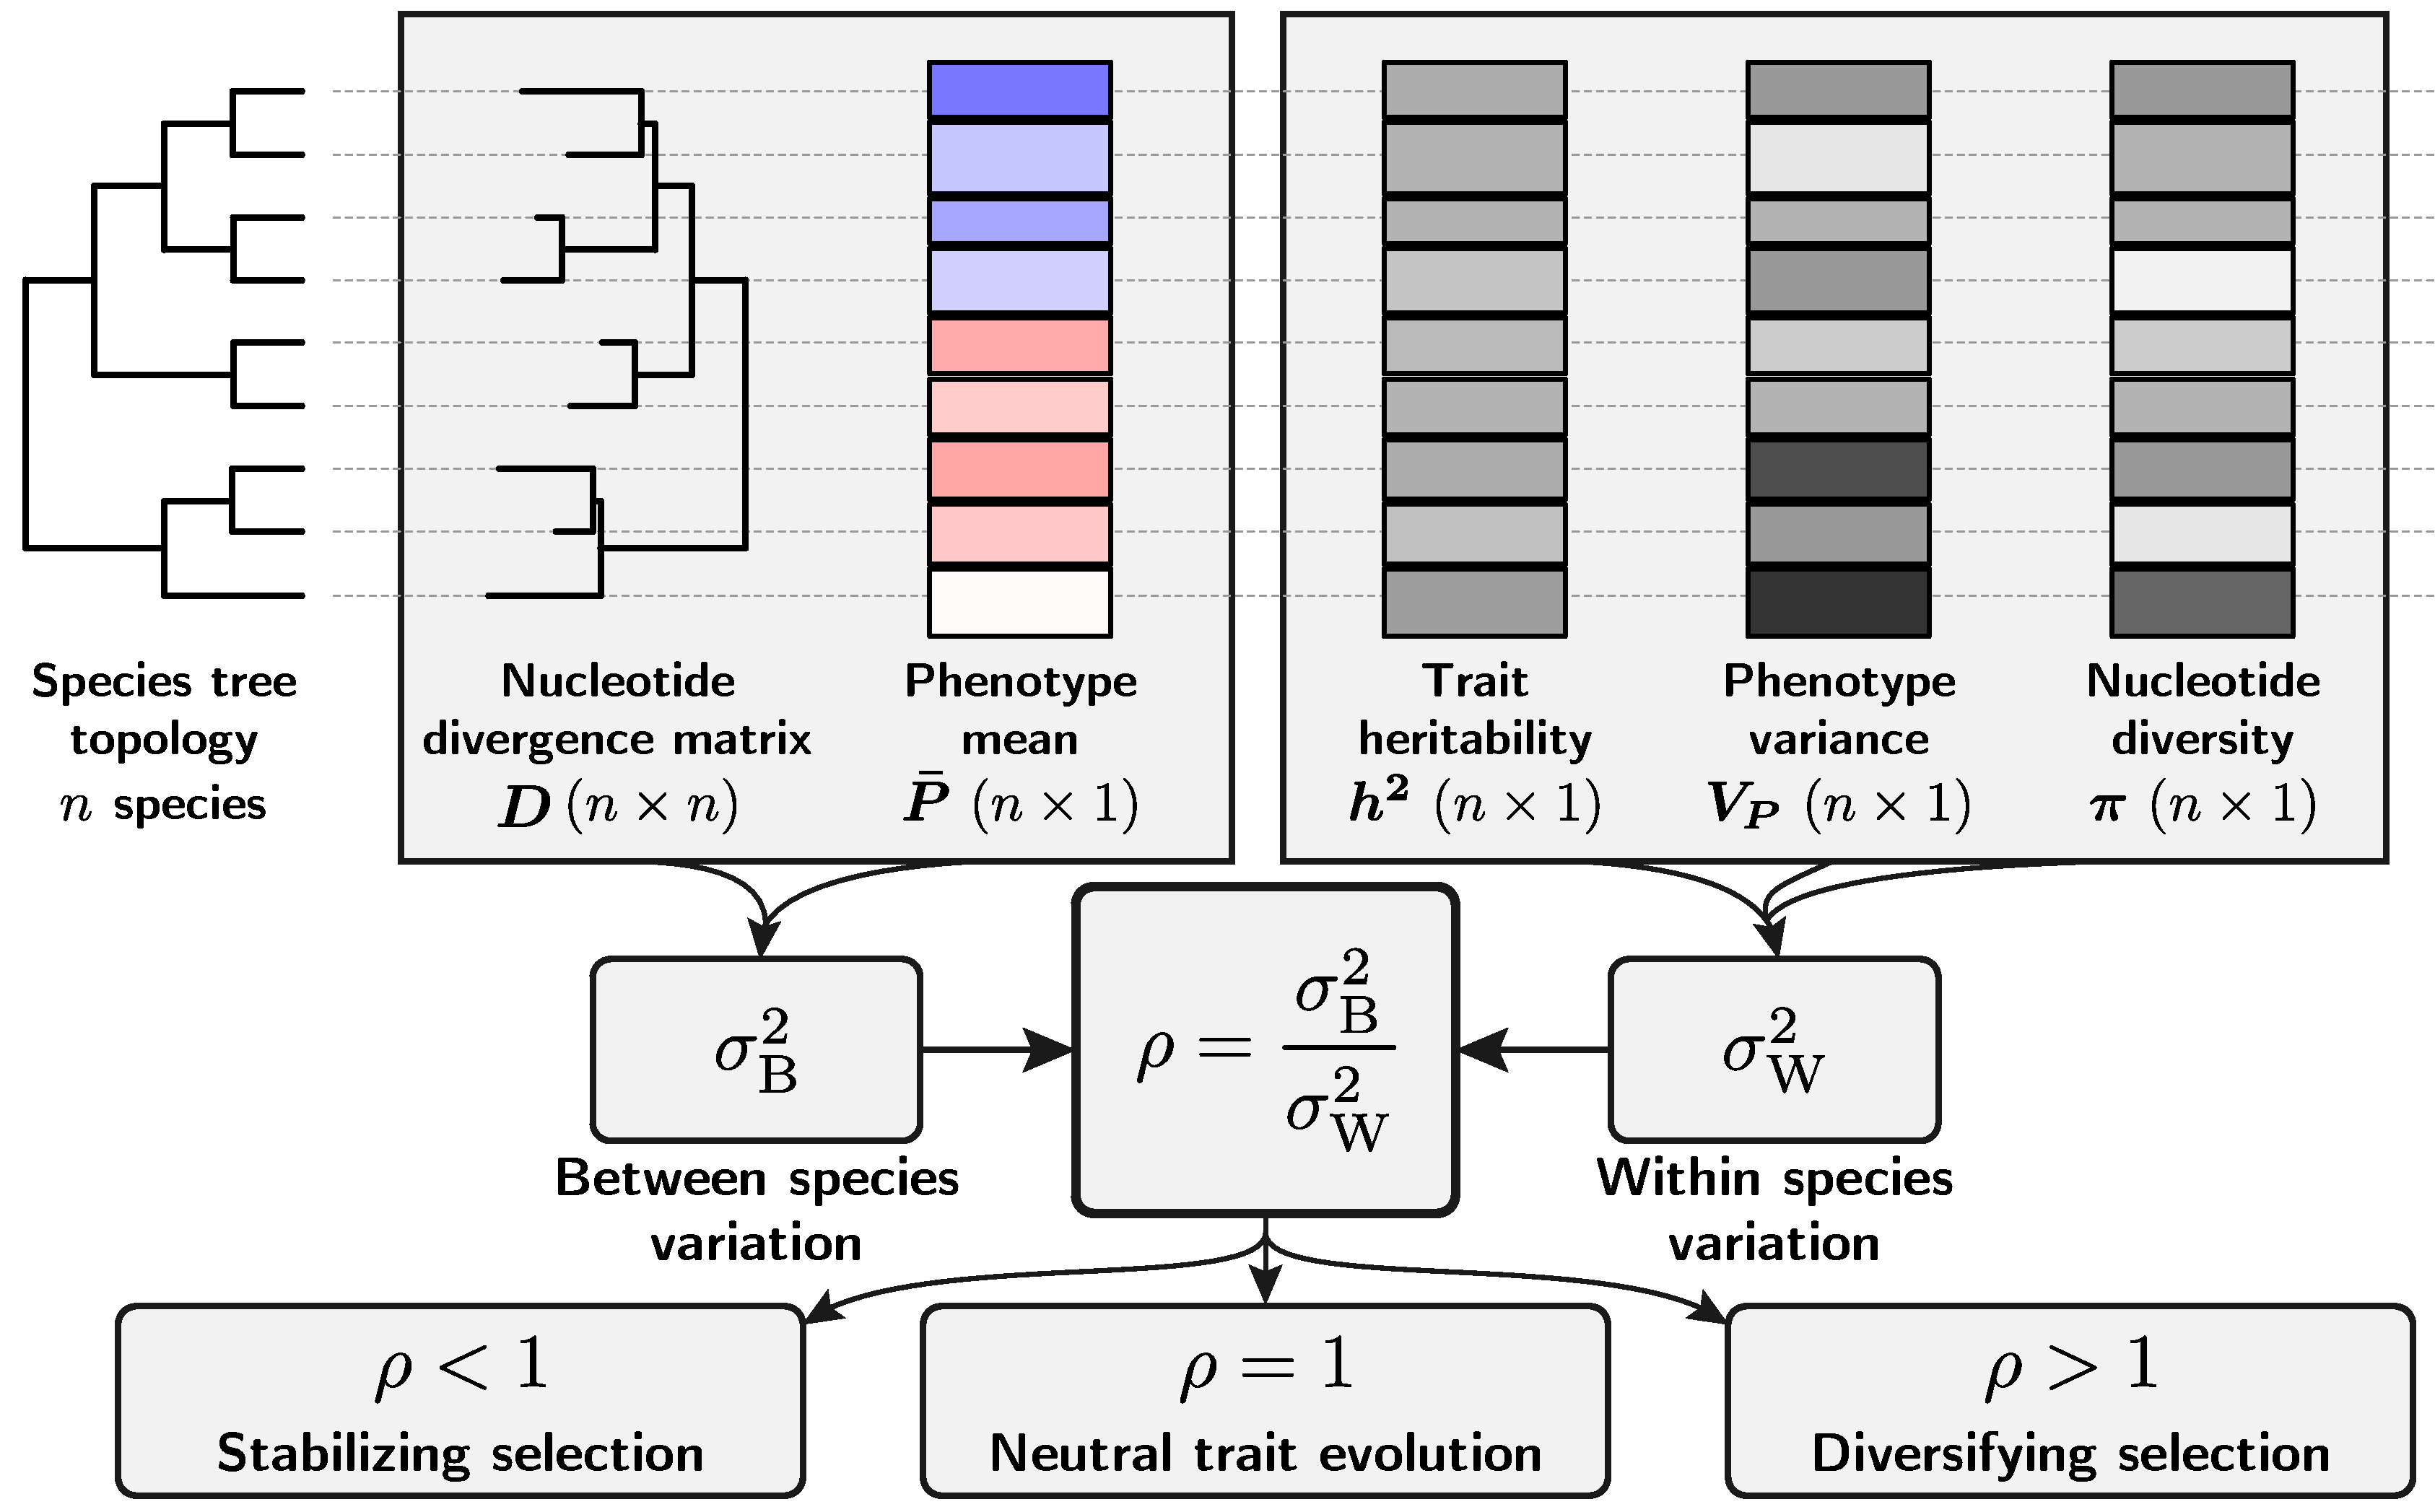
\includegraphics[width=\textwidth, page=1] {figure1}
    \caption{
        Between species, the change along the phylogeny of the mean phenotypic trait allows the estimation of between-species trait variation, $\EstRateBetween$, which is normalized by nucleotide divergence.
        Within species, the genetic variance allows the estimation of within-species trait variation, $\EstRateWhithin$, which is  normalized by nucleotide diversity.
        $\EstNI$ is the ratio of $\EstRateBetween$ over $\EstRateWhithin$.
        Under neutral evolution, $\EstNI$ is expected to be equal to one.
        Under diversifying selection, the trait is heterogeneous between species, but homogeneous within species, leading to $\EstNI$ greater than one.
        Under stabilizing selection, the trait is homogeneous between species, leading to $\EstNI$ smaller than one.
        Importantly, the sequence from which nucleotide diversity and divergence are estimated should be neutrally evolving, but they are not necessarily linked to the quantitative trait under study, they allow for discarding the confounding effect on mutation rate diversity, population size and divergence time.
    }
    \label{fig:methods}
\end{figure*}

\subsubsection*{Neutrality index}

The variability between either individuals or species can be obtained for both quantitative traits and genomic sequences.
At the population level, the variability of the trait between individuals can be combined with the nucleotide diversity of any neutrally evolving genomic region to obtain $\RateWhithin$\DIFdelbegin \DIFdel{, which equals $\RateMut$ if the trait is neutrally evolving (see above)}\DIFdelend .
At the phylogenetic level, the variability of the mean trait value between species can be combined with the nucleotide divergence of any neutrally evolving genomic region to obtain $\RateBetween$.
\DIFdelbegin \DIFdel{Similarly, $\RateBetween=\RateMut$ if }\DIFdelend \DIFaddbegin \DIFadd{If }\DIFaddend the trait is neutrally evolving and the genetic architecture of the trait has not changed along the phylogenetic tree\DIFdelbegin \DIFdel{.
We thus have, for a neutrally evolving trait:
}\begin{gather*}
    \DIFdel{\RateWhithin = \RateBetween \text{ from eq.~\ref{eq:rate-pop} and~\ref{eq:rate-phy}}, }\\
    \DIFdel{\Rightarrow \NI \defEqual \frac{\RateBetween}{\RateWhithin} = 1.
}\end{gather*}%DIFAUXCMD
\DIFdelend \DIFaddbegin \DIFadd{, we thus have:
}\begin{align}
    \DIFadd{\frac{\RateBetween}{\RateWhithin} }&\DIFadd{= \frac{\VarPhy}{4 \NucDiv} \Multiply \frac{\pi}{\Heritability \Multiply \VarPhenotype} \text{ by definition and eq.~\ref{eq:def-rate-pheno-pop} and~\ref{eq:def-rate-phy}},}\\
    &\DIFadd{= \frac{\MutationRatePheno \Multiply \GenArchi}{\MutationRateNuc} \Multiply \frac{\MutationRateNuc}{\MutationRatePheno \Multiply \GenArchi} \text{ from eq.~\ref{eq:rate-pheno-pop} and~\ref{eq:rate-phy}}, }\\
    &\DIFadd{= 1.
}\end{align}\DIFaddend 
We define a neutrality index \DIFdelbegin \DIFdel{$\NI = \RateBetween / \RateWhithin$ that will equal }\DIFdelend \DIFaddbegin \DIFadd{$\NI$ as:
}\begin{align}
\DIFadd{\NI \defEqual \frac{\RateBetween}{\RateWhithin},
}\end{align}
 \DIFadd{which will equal to }\DIFaddend $1$ for a trait evolving neutrally.
Both $\RateBetween$ and $\RateWhithin$ can be estimated using quantitative trait and genomic sequences within and between species, while neither the mutation \DIFdelbegin \DIFdel{rate }\DIFdelend \DIFaddbegin \DIFadd{rates }\DIFaddend ($\MutationRatePheno$ \DIFaddbegin \DIFadd{and $\MutationRateNuc$}\DIFaddend ), nor the effective population size ($\Ne$)\DIFaddbegin \DIFadd{, generation time ($\GenTime$) }\DIFaddend or time of divergence (\DIFdelbegin \DIFdel{$\Time$}\DIFdelend \DIFaddbegin \DIFadd{$\NbrGen$}\DIFaddend ) need to be estimated.
Moreover, the \DIFaddbegin \DIFadd{nucleotide }\DIFaddend sequence from which $\pi$ and \DIFdelbegin \DIFdel{$d$ are estimated }\DIFdelend \DIFaddbegin \DIFadd{$\NucDiv$ are obtained }\DIFaddend should be neutrally evolving, but they are not necessarily linked to the quantitative trait under study.

\subsection*{\DIFdelbegin \DIFdel{Estimate}\DIFdelend \DIFaddbegin \DIFadd{Estimation}\DIFaddend }\label{subsec:estimate}

\DIFdelbegin \DIFdel{Based on the comparative framework that can account for phylogenetic inertia~\mbox{%DIFAUXCMD
\citep{felsenstein_phylogenies_1985, omeara_testing_2006}}\hskip0pt%DIFAUXCMD
}\DIFdelend \DIFaddbegin \DIFadd{We denote $\EstNI$}\DIFaddend , \DIFdelbegin \DIFdel{we }\DIFdelend \DIFaddbegin \DIFadd{$\EstRateBetween$ and $\EstRateWhithin$ the point estimates of respectively $\NI$, $\RateBetween$ and $\RateWhithin$.
For each species with data available, $\RateWhithin$ as defined in eq.~\ref{eq:def-rate-pheno-pop} can be seen as a replicate sample.
Thus, $\EstRateWhithin$ can be obtained by averaging out across all the sampled species.
On the other hand, $\RateBetween$ such as as defined in eq.~\ref{eq:def-rate-phy} only refers to a pair of species, and thus must be generalized to account for different species divergence, as is done in the comparative framework~\mbox{%DIFAUXCMD
\citep{felsenstein_phylogenies_1985, omeara_testing_2006}}\hskip0pt%DIFAUXCMD
.
Generally, $\EstRateWhithin$ can thus be seen as an estimate of the rate of the evolution of the quantitative trait along a phylogeny, when the tree is measured in units of $4d$ ($d$ is the nucleotide divergence).
As such, any phylogenetic comparative methods that allow the estimation of phenotypic rates of evolution on a tree scaled by $4d$, instead of time as is usually the case, can be used to estimate $\EstRateWhithin$.
We }\DIFaddend provide a maximum likelihood estimate for $\NI$ as well as a Bayesian estimate to derive posterior probabilities that the null model of neutrality (i.e.~$\NI = 1$) is rejected.

\subsubsection*{Maximum likelihood estimate}
At the phylogenetic scale, for $\NbrTaxa$ taxa in the tree, $\DistanceMatrix$ ($\NbrTaxa \times \NbrTaxa$) is the \DIFaddbegin \DIFadd{symmetric }\DIFaddend distance matrix computed from the branch lengths \DIFdelbegin \DIFdel{($d$ as nucleotide divergence in units of substitutions per site) }\DIFdelend and the topology of the phylogenetic tree.
The diagonal $\Distance_{\Spi,\Spi}$ represents the total \DIFdelbegin \DIFdel{distances }\DIFdelend \DIFaddbegin \DIFadd{nucleotide divergence }\DIFaddend from the root of the tree to each taxon ($\Spi$).
The off-diagonal elements (\DIFdelbegin \DIFdel{$\Distance_{\Spi,\Spj} = \Distance_{\Spj,\Spi}$}\DIFdelend \DIFaddbegin \DIFadd{$\Distance_{\Spi,\Spj} = \NucDiv$}\DIFaddend ) are the distances between the root and the most recent common ancestor of taxa $\Spi$ and $\Spj$\DIFaddbegin \DIFadd{, as in equation~\ref{eq:distance}}\DIFaddend .
The state $\RootTrait$ at the root of the tree for the trait can be estimated from the $\NbrTaxa \times 1$ vector of mean trait values $\VecTrait$ at the tips of the tree using maximum likelihood~\citep{omeara_testing_2006}:
\begin{gather}
    \RootTrait = \left( \VecOne\tr \MultiplyMatrix \DistanceMatrix\inv \MultiplyMatrix \VecOne \right)\inv \Multiply \left( \VecOne\tr \MultiplyMatrix \DistanceMatrix\inv \MultiplyMatrix \VecTrait \right), \label{eq:estimated-root-trait}
\end{gather}
where $\VecOne$ is an $\NbrTaxa \times 1$ column vector of ones.

Finally, between-species variation $\EstRateBetween$ is estimated as~\citep{omeara_testing_2006}:
\begin{gather}
    \EstRateBetween = \frac{1}{4}\frac{\left( \VecTrait -  \RootTrait \Multiply \VecOne \right)\tr \MultiplyMatrix \DistanceMatrix\inv \MultiplyMatrix \left( \VecTrait -  \RootTrait \Multiply \VecOne  \right)}{\NbrTaxa - 1}. \label{eq:estimated-rate-phy}
\end{gather}

For a given species $\Spi$ with inter-individual data available, additive genetic variance of a trait ($\VarGeneticSpi$) is the product of heritability ($\Heritability_{i}$) and phenotypic variance ($V_{\Trait, i}$).
The ratio of $\VarGeneticSpi$ over nucleotide diversity of neutrally evolving sequences ($\pi_{\Spi}$) is a sample estimate of $\RateWhithin$.
Averaged across all species, we obtain the estimate $\EstRateWhithin$ as:
\begin{gather}
    \EstRateWhithin = \dfrac{1}{\NbrTaxa}\sum_{i=1}^{\NbrTaxa}\frac{  \VarGeneticSpi}{ \pi_{i}} = \dfrac{1}{\NbrTaxa}\sum_{i=1}^{\NbrTaxa} \frac{  V_{\Trait, i} \Multiply \Heritability_{i}}{ \pi_{i}}. \label{eq:estimated-rate-pop}
\end{gather}

As depicted in fig.~\ref{fig:methods}, the neutrality index is estimated as:
\begin{gather}
    \EstNI = \frac{\EstRateBetween}{\EstRateWhithin}. \label{eq:estimated-NI}
\end{gather}

\subsubsection*{\DIFdelbegin \DIFdel{Bayesian estimate}\DIFdelend \DIFaddbegin \DIFadd{Multivariate Brownian process}\DIFaddend }

\DIFdelbegin \DIFdel{The Bayesian framework allows obtaining the posterior distribution of the neutrality index (}\DIFdelend \DIFaddbegin \DIFadd{In the previous section, }\DIFaddend $\EstNI$ \DIFdelbegin \DIFdel{) for a given trait.
Even though $\EstNI$ }\DIFdelend is estimated independently for each trait of interest\DIFdelbegin \DIFdel{in the maximum likelihood framework (previous section), here }\DIFdelend \DIFaddbegin \DIFadd{.
Here }\DIFaddend we generalize to $\Ntrait$ traits co-varying along the phylogenetic tree\DIFdelbegin \DIFdel{using the }\textit{\DIFdel{BayesCode}} %DIFAUXCMD
\DIFdel{software~\mbox{%DIFAUXCMD
\citep{latrille_inferring_2021}}\hskip0pt%DIFAUXCMD
}\DIFdelend .
Trait variation along the phylogenetic tree is modeled as a $\Ntrait$-dimensional Brownian process $\Brownian$ ($1 \times \Ntrait$) starting at the root and branching along the tree topology~\citep{huelsenbeck_detecting_2003, lartillot_phylogenetic_2011, lartillot_joint_2012, latrille_inferring_2021}.
The rate of change of the Brownian process is determined by the positive semi-definite and symmetric covariance matrix between traits $\CovarianceMatrix$ ($\Ntrait \times \Ntrait$).
The \DIFaddbegin \DIFadd{branch length of the tree on which the Brownian process runs is measured in units of $4d$ ($d$ is the nucleotide divergence).
The }\DIFaddend off-diagonal elements of $\CovarianceMatrix$ are the covariance between traits, and the diagonal elements are the variance of each trait \DIFdelbegin \DIFdel{, thus corresponding }\DIFdelend \DIFaddbegin \DIFadd{when measured in $4d$ units, and thus equate }\DIFaddend to $\EstRateBetween$ (see section~S\ref{subsec:multivariate-brownian-process}).
\DIFaddbegin 


\subsubsection*{\DIFadd{Bayesian estimate}}
\DIFadd{The Bayesian framework allows obtaining the posterior distribution of neutrality index ($\EstNI$) for traits of interest.
We used the }\textit{\DIFadd{BayesCode}} \DIFadd{software to model $\Ntrait$-dimensional Brownian processes along a phylogenetic tree~\mbox{%DIFAUXCMD
\citep{latrille_inferring_2021}}\hskip0pt%DIFAUXCMD
.
}\DIFaddend With an inverse Wishart distribution as the {prior} on the covariance matrix, the {posterior} on $\CovarianceMatrix$, conditional on $\brownian$ is also an invert Wishart distribution (see section~S\ref{subsec:sampling-the-covariance-matrix}).
We used Metropolis-Hastings algorithm to sample $\Brownian$, while the posterior distribution of $\CovarianceMatrix$ is sampled using Gibbs sampling.
For each trait and each species, the prior on heritability ($\Heritability$) for each species is set as a uniform distribution with user-defined boundaries.
Heritability and phenotypic variance for each trait are combined with nucleotide diversity to compute $\EstRateWhithin$ for each species before being averaged across species (as in eq.~\ref{eq:estimated-rate-pop}).
From $\EstRateWhithin$ and $\CovarianceMatrix$, the posterior distribution of $\EstNI$ (as in eq.~\ref{eq:estimated-NI}) is obtained for each trait.
The posterior distribution of $\EstNI$ thus allows testing for deviation from neutrality (Fig.~\ref{fig:methods}), for example, by computing $\proba [\EstNI > 1 ]$ to test for evidence of diversifying selection and $\proba [\EstNI < 1 ]$ to test for evidence of stabilizing selection.

\subsubsection*{Applicability to empirical data}

Our method assumes that the narrow-sense heritability ($\Heritability$) of a trait is known such as to estimate additive genetic variance ($\VarGenetic$) from phenotypic variance ($\VarPhenotype$) as $\VarGenetic = \Heritability \Multiply \VarPhenotype$.
Fortunately, if heritability is not known, the test for diversifying selection can still be performed, although it is underpowered.
Indeed, if the additive genetic variance is substituted by phenotypic variance, it is equivalent to assuming complete heritability ($\Heritability = 1$).
Because $\Heritability \leq 1$ by definition, we overestimate the within-species variation and thus underestimate $\EstNI$.
It is, however, possible to test for diversifying selection because testing for $\EstNI > 1$ while using phenotypic variance instead of additive genetic variance means that knowing the additive genetic variance would have only increased the evidence for diversifying selection.
\DIFdelbegin \DIFdel{Similarly, }\DIFdelend \DIFaddbegin \DIFadd{Additionally, empirical estimates of $\Heritability$ are surprisingly stable across species and falling within the range of 0.2-0.5 in a vast majority of phenotypes tested~\mbox{%DIFAUXCMD
\citep{hansen_heritability_2011, hansen_evolvability_2021}}\hskip0pt%DIFAUXCMD
.
Alternatively, }\DIFaddend using the broad-sense heritability ($H^2$) instead of narrow-sense heritability ($\Heritability$) results in an underestimation of $\EstNI$ since $\Heritability \leq H^2$.
\DIFdelbegin \DIFdel{In contrast}\DIFdelend \DIFaddbegin \DIFadd{If available, such prior knowledge on $\Heritability$ can be leveraged instead of assuming complete heritability to increase the statistical power to detect diversifying selection.
}

\DIFadd{In contrast to the test of diversifying selection}\DIFaddend , the test for stabilizing selection is invalid if $\EstNI$ is underestimated.
Several assumptions made by our test might not hold on empirical data and their consequences on the neutrality index and the test that can be performed are shown in Table~\ref{table:assumptions}.

\subsection*{Simulation}\label{subsec:simulations}

% vG: 13.8, vP: 69.0, vE: 55.2, nbr_loci: 5000, a: 1.0, mut_rate: 1.38e-05, pop_size: 50, h2: 0.2
% pS = 0.0027577478571428568
% Tree length (dS) = 2.340579
% Tree length (My) = 1259.4490200000002
% Root age (My) = 98.9489413888889
% Root age (dS) = 0.18388820079995308
% nbr_sites_var = 27.577478571428568
% u = 1.3788739285714283e-05
% nbr_generations = 13336.114128321291
We tested the performance of our neutrality index ($\NI$) to detect selection on a quantitative trait using simulations.
We performed simulations under different selective regimes (neutral, stabilizing, diversifying), different demographic histories (constant or fluctuating population size) and different evolution of the mutation rate (constant or fluctuating).
Simulations were individual-based and followed a Wright-Fisher model with mutation, selection and drift for a diploid population including speciation along a predefined ultrametric phylogenetic tree (Fig.~\ref{fig:simulator}A\&B).
Each individual phenotypic value was the sum of genotypic value and an environmental effect.
The environmental effect was normally distributed with variance $\VarEnv$.
We assumed that the genotypic value was encoded by $\NbrLoci=5,000$ loci, with each locus contributing an additive effect that was normally distributed with standard deviation $a=1$ (Fig.~\ref{fig:simulator}A and \DIFaddbegin \DIFadd{for the theoretical formulation see }\DIFaddend section~S\ref{subsec:genotype-phenotype-map} \DIFdelbegin \DIFdel{for theoretical formulation}\DIFdelend \DIFaddbegin \DIFadd{and fig.~\ref{fig:simulator-summary}}\DIFaddend ).
We assumed a trait with a narrow-sense heritability of $\Heritability=0.2$ and computed the theoretical $\VarEnv$ accordingly (see section~S\ref{subsec:genotype-phenotype-map}).
Assuming a diploid panmictic population of size $\Ne=50$ at the root of the tree, and with non-overlapping generations, we simulated explicitly each generation along an ultrametric phylogenetic tree.
For each offspring, the number of mutations was drawn from a Poisson distribution with mean $2 \Multiply \MutationRatePheno \Multiply \NbrLoci $, with the mutation rate per \DIFaddbegin \DIFadd{locus per }\DIFaddend generation $\MutationRatePheno$.
From the empirical mammalian dataset (see next section), we computed an average nucleotide divergence from the root to leaves of $0.18$ and average genetic diversity of $0.00276$.
We scaled parameters in our simulations to fit plausible values for mammals.
We thus used a \DIFaddbegin \DIFadd{nucleotide }\DIFaddend mutation rate of \DIFdelbegin \DIFdel{$\MutationRatePheno=0.00276 / 4 \Ne = 1.38 \times 10^{-5}$ }\DIFdelend \DIFaddbegin \DIFadd{$\MutationRateNuc=0.00276 / 4 \Ne = 1.38 \times 10^{-5}$ }\DIFaddend per generation per locus and a total of \DIFdelbegin \DIFdel{$\Time = 0.18 / 1.38 \times 10^{-5} = 13,500$ }\DIFdelend \DIFaddbegin \DIFadd{$0.18 / 1.38 \times 10^{-5} = 13,500$ }\DIFaddend generations from root to leaves, and the number of generations along each branch was proportional to the branch length.
\DIFaddbegin \DIFadd{We set $\MutationRatePheno=\MutationRateNuc$ without loss in generality since the genetic architecture ($\NbrLoci$ and $a$) is assumed constant in the simulator.
}\DIFaddend 

The changes in \DIFdelbegin \DIFdel{log-}\DIFdelend $\MutationRatePheno$ and \DIFdelbegin \DIFdel{log-}\DIFdelend $\Ne$ along the lineages were both modeled by a \DIFdelbegin \DIFdel{geometric Brownian process (}\DIFdelend \DIFaddbegin \DIFadd{Brownian process on the log scale (log-$\MutationRatePheno$ and log-$\Ne$), leading to geometric Brownian motion on the linear scale ($\MutationRatePheno$ and $\Ne$).
These processes are parameterized as }\DIFaddend $\brownian \left(0, \sigma_{\MutationRatePheno}=0.0086\right)$ and $\brownian \left(0, \sigma_{\Ne}=0.0086\right)$, which \DIFdelbegin \DIFdel{led }\DIFdelend \DIFaddbegin \DIFadd{if counted across $13,500$ generations leads }\DIFaddend to a standard deviation of $0.0086 \Multiply \sqrt {13,500} = 1.0$\DIFdelbegin \DIFdel{in log-space from root to leaves}\DIFdelend \DIFaddbegin \DIFadd{.
In other words, the deviation in log-$\Ne$ and log-$\MutationRatePheno$  between the extant species and the root is $1.0$}\DIFaddend .
An Ornstein-Uhlenbeck process was overlaid to the instant value of log-$\Ne$ provided by the geometric Brownian process to account for short-term changes between generations ($\text{OU} \left(0, \sigma_{\Ne}=0.1, \theta_{\Ne}=0.9\right)$).
The geometric Brownian motion accounted for long-term fluctuations (low rate of changes $\sigma_{\Ne}$ but unbounded), while the Ornstein-Uhlenbeck introduced short-term fluctuations (high rate of changes $\sigma_{\Ne}$ but bounded and mean-reverting).
The simulation started from an initial sequence at equilibrium at the root of the tree and, at each node, the process was split until it finally reached the leaves of the tree.
From a speciation process perspective, this was equivalent to an allopatric speciation over one generation.

\DIFdelbegin \DIFdel{A random genetic drift was introduced by resampling individuals at }\DIFdelend \DIFaddbegin \DIFadd{At }\DIFaddend each generation, \DIFdelbegin \DIFdel{with each parent having a probability of being sampled that was proportional to its }\DIFdelend \DIFaddbegin \DIFadd{parents were randomly sampled with a weight proportional to their }\DIFaddend fitness ($W$).
Selection was modeled as a one-dimensional Fisher's geometric landscape, with the fitness of an individual being a monotonously decreasing function of the distance between the individual and the optimal phenotype~\citep{tenaillon_utility_2014,blanquart_epistasis_2016}.
More specifically, the fitness of an individual was given by $W = \e^{(\Trait - \lambda)^2/ \alpha}$, where $\Trait$ was the trait value of the individual, $\lambda=0.0$ was the optimal trait value, and $\alpha=0.02$ was the strength of selection.
Mutations were considered as a displacement of the phenotype in the multidimensional space.
Beneficial mutations moved the phenotype closer to the optimum, while deleterious mutations moved it further away.
Stabilizing selection was implemented by fixing the optimum phenotype to a single value ($\lambda=0.0$).
Diversifying selection was implemented by allowing the optimum phenotype to move along the phylogenetic tree as a geometric Brownian process~\citep{hansen_stabilizing_1997} ($\lambda \sim \brownian \left(0, \sigma_{\lambda}=1.0\right)$).
Neutral evolution was implemented by fixing the fitness landscape ($W=1$), which meant that each individual had the same probability of being sampled at each generation.

Nucleotide diversity ($\pi$) was measured as the heterozygosity of neutral markers that were simulated along the phylogenetic tree but not linked to the trait simulated.
Nucleotide divergence ($d$) was measured as the number of substitutions per site of neutral markers along the branches of the phylogenetic tree.
The additive genetic variance was measured as phenotypic variance multiplied by heritability.
Heritability was estimated from the slopes of the regression of offspring's phenotypic trait values on parental phenotypic trait values~\citep{lynch_genetics_1998} averaged over the last 10 simulated generations.
Heritability was thus not a given parameter of the simulations, but rather measured as it would be in empirical data.

\begin{figure*}[!ht]
    \centering
    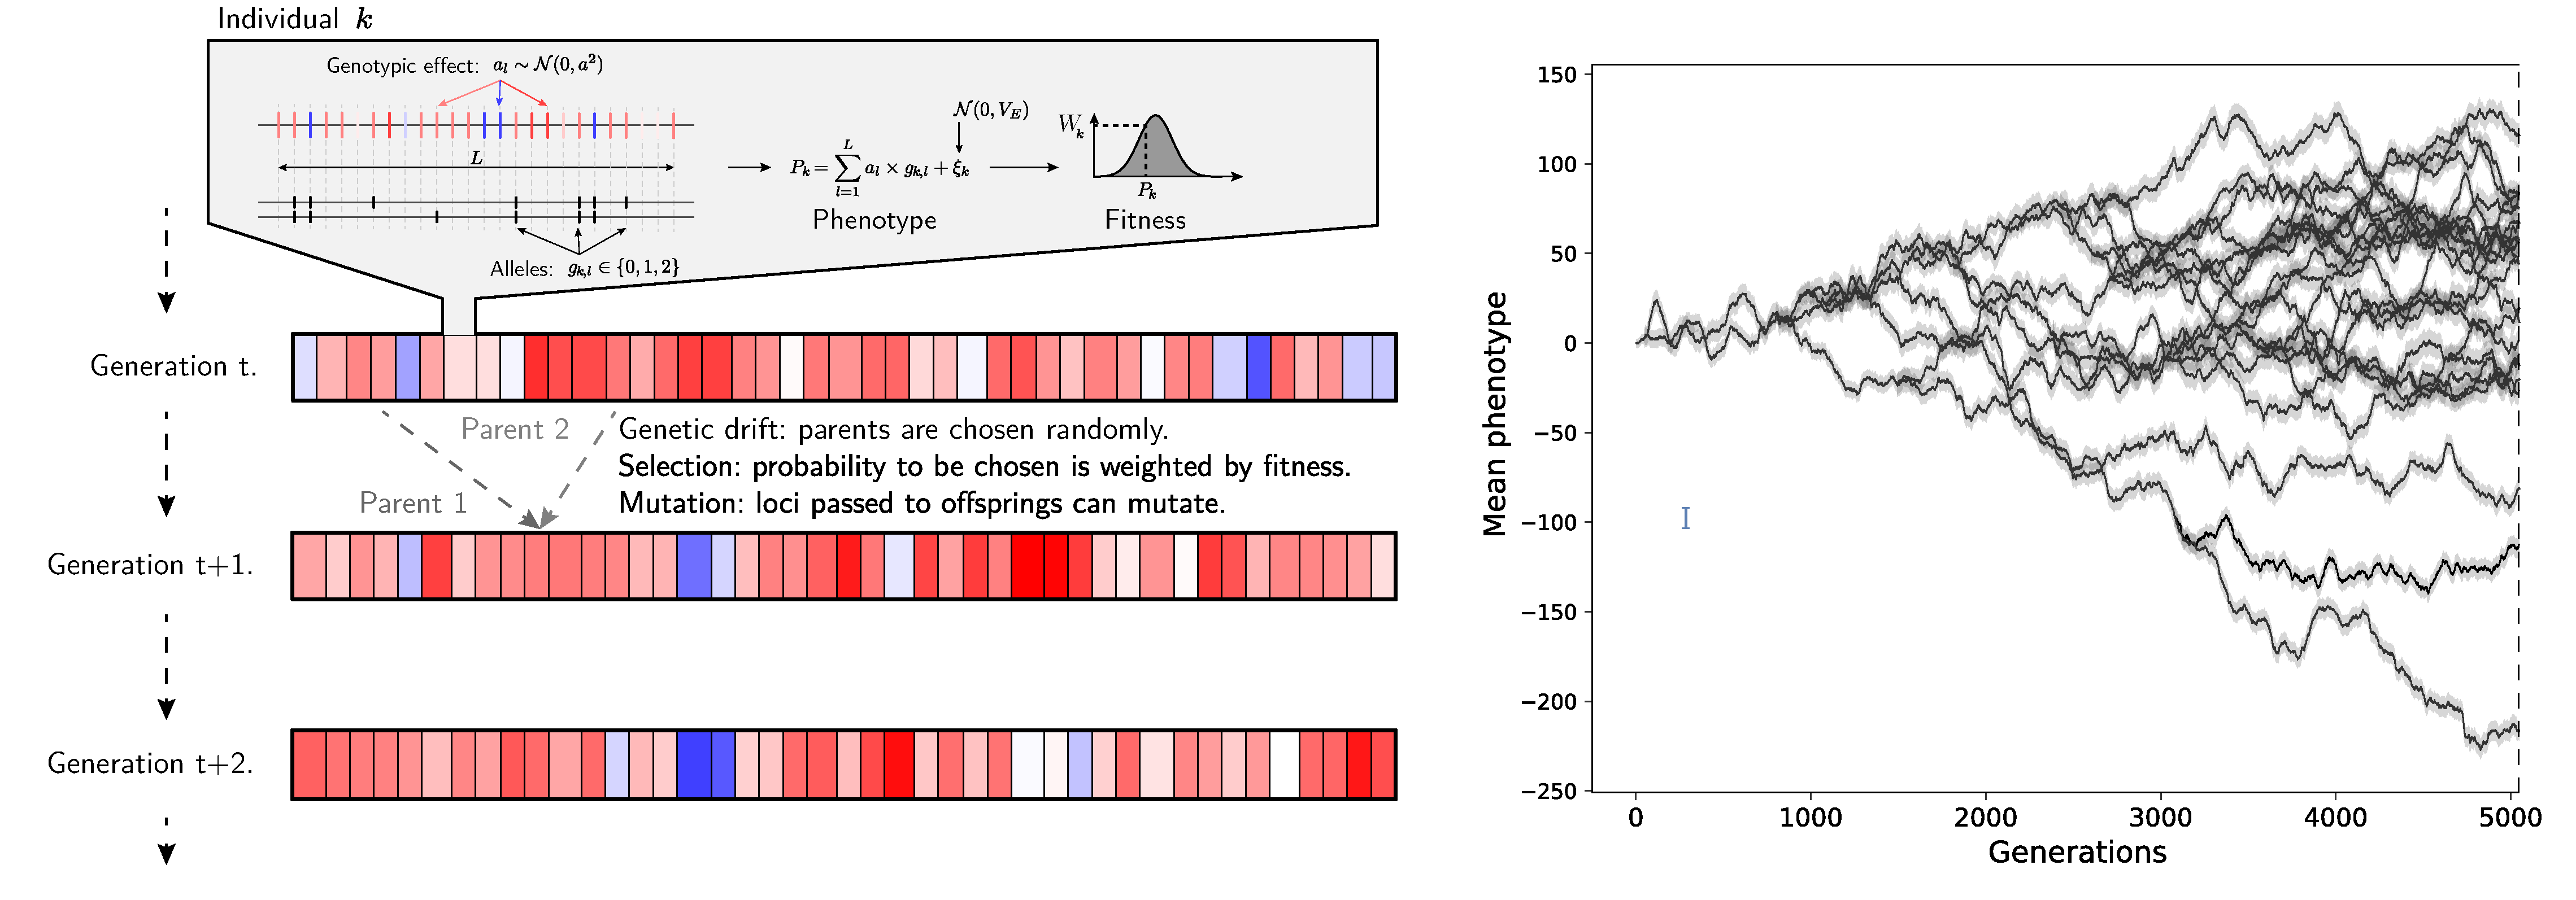
\includegraphics[width=\textwidth, page=1] {figure2}
    \caption{
        Wright-Fisher simulations with mutation, selection and drift.
        Left panel: For a given individual, the trait phenotypic value is the sum of genotypic value and a environmental effect (standard deviation $\VarEnv$).
        The trait's genotypic value is encoded by $\NbrLoci$ \DIFaddbeginFL \DIFaddFL{independent }\DIFaddendFL loci \DIFaddbeginFL \DIFaddFL{(meaning no linkage)}\DIFaddendFL , with each locus contributing additively to the genotypic value.
        Parents are selected for reproduction to the next generation according to their phenotypic value, with a probability proportional to their fitness.
        Mutations are drawn from a Poisson distribution, with each locus having a probability $\MutationRatePheno$ to mutate.
        Drift is modeled by the resampling of parents.
        Right panel: examples of a trait evolving along a phylogenetic tree, with the mean phenotype (black line) and the variance of the trait genotypic value (gray area).
    }
    \label{fig:simulator}
\end{figure*}

\subsection*{Empirical dataset}\label{subsec:empirical-dataset}

We analyzed a dataset of body and brain masses from mammals.
The log-transformed values of body and brain masses were taken from \citet{tsuboi_breakdown_2018}.
We removed individuals not marked as adults and split the data into males and females due to sexual dimorphism in body and brain masses.
We discarded species with only one representative \DIFdelbegin \DIFdel{sample}\DIFdelend \DIFaddbegin \DIFadd{since phenotypic variance cannot be estimated}\DIFaddend .
The mammalian \DIFdelbegin \DIFdel{nucleotide diversity was obtained }\DIFdelend \DIFaddbegin \DIFadd{genomic data are gathered }\DIFaddend from the Zoonomia project~\citep{genereux_comparative_2020}\DIFdelbegin \DIFdel{, with nucleotide divergence obtained }\DIFdelend \DIFaddbegin \DIFadd{.
More specifically, nucleotide divergence is estimated }\DIFaddend on a set of neutral markers in \citet{foley_genomic_2023}, and with nucleotide diversity measured as heterozygosity in \citet{wilder_contribution_2023}.

We also analyzed a dataset of primate species, with the nucleotide variation obtained from \citet{kuderna_global_2023} and the quantitative trait variation also from \citet{tsuboi_breakdown_2018}, using the same filtering as for the mammalian dataset.
However, the primate nucleotide divergence was not obtained on a set of neutral markers as for the mammalian dataset, but across the whole genome.
\DIFaddbegin \DIFadd{As such, the evidence for $\EstNI > 1$ does not necessarily imply that the trait is evolving under diversifying selection since non-neutral markers for divergence can lead to a spurious $\EstNI > 1$ (see table~\ref{table:assumptions}).
}\DIFaddend 

\section*{Results}\label{sec:results}

\subsection*{Neutrality index}

For a neutral trait, the genetic architecture, meaning the number of loci encoding the trait and the average effect of a mutation on the trait, is formally related to both within and between-species variation of the trait.
We defined the neutrality index as $\NI = \RateBetween/\RateWhithin$, which equals $1$ for a neutral trait (see Materials and Methods), suggesting that traits for which this relationship was not verified were putatively under selection.
Under stabilizing selection, the variation between species is depleted because the mean trait value is maintained \DIFdelbegin \DIFdel{similar }\DIFdelend \DIFaddbegin \DIFadd{toward similar values }\DIFaddend between different species, which leads to $\NI < 1$.
In contrast, under diversifying selection, the variation between species is inflated because species will have potentially different trait values~\citep{hansen_stabilizing_1997}, which leads to $\NI > 1$.
Our neutrality index for a quantitative trait leveraged the data for any number of species, and took advantage of the signal over the whole phylogenetic tree, while at the same time taking into account phylogenetic inertia and addressing the non-independence between species (Fig.~\ref{fig:methods}).
This statistic was obtained as a maximum likelihood estimate ($\EstNI$), from eq.~\ref{eq:estimated-rate-pop} and~\ref{eq:estimated-rate-phy}.
We also devised a Bayesian estimate to obtain the posterior distribution of the neutrality index, and test for diversifying selection as $\proba [\EstNI > 1]$, and stabilizing selection as $\proba [\EstNI < 1]$.

Our neutrality index made a series of assumptions that we described in details in the Material and Methods section.
Table\DIFaddbegin \DIFadd{~}\DIFaddend \ref{table:assumptions} summarized these assumptions and outlined possible consequences for the neutrality test that we proposed.

\subsection*{Results against simulations}\label{subsec:results-against-simulations}

The inference framework was first tested on independently simulated datasets matching an empirically relevant mammalian empirical regime (see Materials and Methods).
Under constant population size ($\Ne$) and constant mutation \DIFdelbegin \DIFdel{rate }\DIFdelend \DIFaddbegin \DIFadd{rates }\DIFaddend ($\MutationRatePheno$ \DIFaddbegin \DIFadd{and $\MutationRateNuc$}\DIFaddend ) across the phylogenetic tree (fig.~\ref{fig:results-simulations}, top row), we found no false negative for simulations of stabilizing ($\proba [\EstNI < 1] > 0.975$; blue in fig.~\ref{fig:results-simulations}) or diversifying ($\proba [\EstNI > 1] > 0.975$; red in fig.~\ref{fig:results-simulations}) selection.
For simulations under neutral evolution, 77\% of those were correctly identified ($0.025 \leq \proba [\EstNI > 1] \leq 0.975$; yellow in fig.~\ref{fig:results-simulations}), while 21\% and 2\% were wrongly detected as stabilizing or diversifying selection, respectively.
Once we introduced fluctuating $\Ne$\DIFdelbegin \DIFdel{and }\DIFdelend \DIFaddbegin \DIFadd{, }\DIFaddend $\MutationRatePheno$ \DIFaddbegin \DIFadd{and $\MutationRateNuc$}\DIFaddend (Fig.~\ref{fig:results-simulations}, bottom row), our ability to identify simulations under either diversifying or stabilizing selection remained the same with all cases detected correctly.
For simulations under neutral evolution, 51\% of the simulations were correctly detected ($0.025 \leq \proba [\EstNI > 1] \leq 0.975$), while 49\% were detected as stabilizing selection ($\proba [\EstNI < 1] > 0.975$) and none as diversifying selection.

\begin{figure*}[!ht]
    \centering
    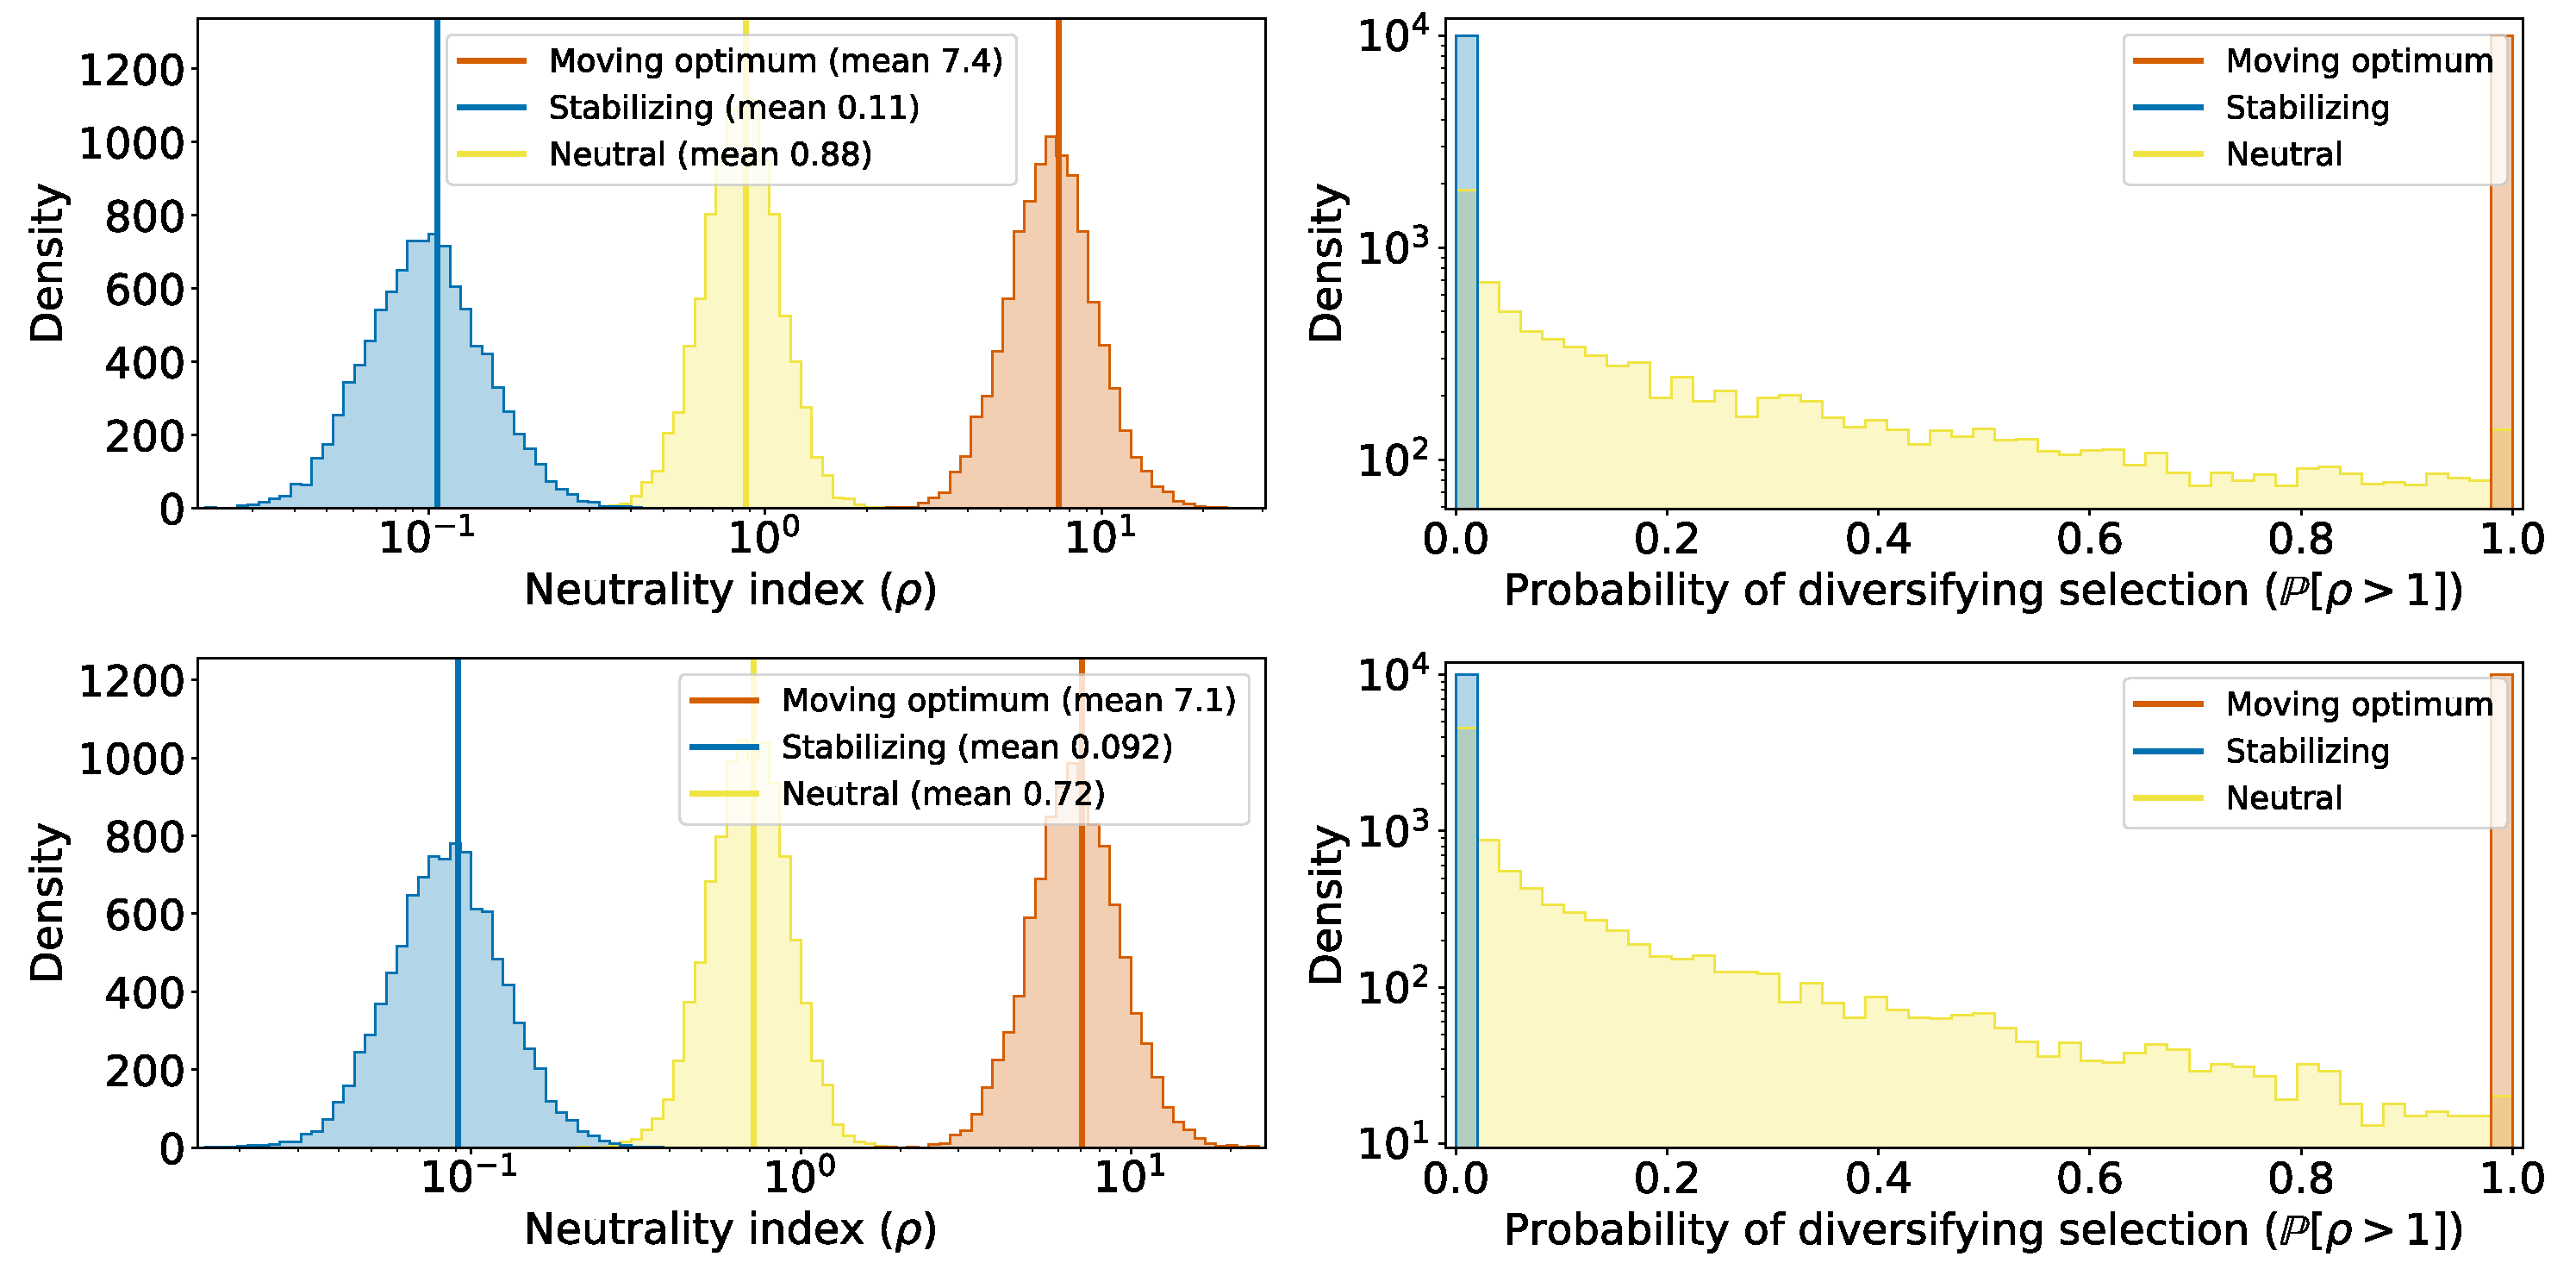
\includegraphics[width=\textwidth, page=1] {figure3}
    \caption{
        $10,000$ simulations of trait evolution along a phylogenetic tree under different selection regimes.
        Traits simulated under stabilizing selection (blue), under a neutral evolution (yellow), and under a moving optimum (red).
        Histogram of ratio of between-species trait variation ($\EstRateBetween$) over within-species trait variation $\EstRateWhithin$ with $\EstNI = \EstRateBetween / \EstRateWhithin$ estimated from each simulated data (left) and probabilities of $\EstNI$ being greater than $1$ (right).
        Effective population size ($\Ne$) and mutation \DIFdelbeginFL \DIFdelFL{rate }\DIFdelendFL \DIFaddbeginFL \DIFaddFL{rates }\DIFaddendFL ($\MutationRatePheno$ \DIFaddbeginFL \DIFaddFL{and $\MutationRateNuc$}\DIFaddendFL ) were either constant (top row), or fluctuating as a Brownian process along the phylogenetic tree (bottom row).
    }
    \label{fig:results-simulations}
\end{figure*}


\begin{table*}[t!]
    \centering
    \begin{adjustbox}{width = 0.75\textwidth}
        \begin{tabular}{||l|l|l|c|c|c|c|c||}
        \toprule
        Dataset & Trait & $\Heritability$ & Sex & $\NbrTaxa$ & $\EstNI$ & $95\%$ CI for $\EstNI$ & $\proba [\EstNI > 1 ]$ \\ \hline
        \midrule
        Mammals & Body mass & 1.0 & \Male & 36 & 0.340 & 0.217-0.523 & 0.000 \\ \hline
        Mammals & Body mass & 1.0 & \Female & 26 & 0.277 & 0.160-0.490 & 0.000 \\ \hline
        Mammals & Body mass & $\mathcal{U}(0.2, 0.4)$ & \Male & 36 & 1.124 & 0.721-1.754 & 0.635 \\ \hline
        Mammals & Body mass & $\mathcal{U}(0.2, 0.4)$ & \Female & 26 & 0.936 & 0.523-1.715 & 0.324 \\ \hline \hline
        Mammals & Brain mass & 1.0 & \Male & 36 & 1.351 & 0.851-2.173 & 0.877 \\ \hline
        Mammals & Brain mass & 1.0 & \Female & 26 & 1.727 & 0.991-2.938 & 0.972 \\ \hline
        Mammals & Brain mass & $\mathcal{U}(0.2, 0.4)$ & \Male & 36 & 4.527 & 2.831-7.091 & 1.000 \\ \hline
        Mammals & Brain mass & $\mathcal{U}(0.2, 0.4)$ & \Female & 26 & 6.001 & 3.288-10.941 & 1.000 \\ \hline \hline
        Primates & Body mass & 1.0 & \Male & 71 & 0.558 & 0.401-0.784 & 0.000 \\ \hline
        Primates & Body mass & 1.0 & \Female & 65 & 0.389 & 0.278-0.547 & 0.000 \\ \hline
        Primates & Body mass & $\mathcal{U}(0.2, 0.4)$ & \Male & 71 & 1.875 & 1.288-2.695 & 1.000 \\ \hline
        Primates & Body mass & $\mathcal{U}(0.2, 0.4)$ & \Female & 65 & 1.296 & 0.899-1.821 & 0.914 \\ \hline \hline
        Primates & Brain mass & 1.0 & \Male & 71 & 1.929 & 1.395-2.616 & 1.000 \\ \hline
        Primates & Brain mass & 1.0 & \Female & 65 & 1.950 & 1.399-2.790 & 1.000 \\ \hline
        Primates & Brain mass & $\mathcal{U}(0.2, 0.4)$ & \Male & 71 & 6.479 & 4.658-8.944 & 1.000 \\ \hline
        Primates & Brain mass & $\mathcal{U}(0.2, 0.4)$ & \Female & 65 & 6.522 & 4.664-9.294 & 1.000 \\
        \bottomrule
        \end{tabular}
    \end{adjustbox}
    \caption{
    Test of diversifying selection on a mammal and a primate dataset, by splitting males (\Male) and females (\Female).
    Traits considered were body mass or brain mass (log-transformed).
    Heritability ($\Heritability$) was either assumed complete ($\Heritability=1.0$) or uniformly distributed between 20\% and 40\%  ($\Heritability \sim \mathcal{U}(0.2, 0.4)$).
    $\NbrTaxa$ was the number of species in the dataset.
    $\EstNI$ was the posterior estimate of our neutrality index, with the $95\%$ credible interval (CI) for $\EstNI$ also computed.
    $\proba [\EstNI > 1 ]$ was the estimated posterior probability of diversifying selection.
    }
    \label{table:empirical}
\end{table*}

\subsection*{Results on empirical data}\label{subsec:results-on-empirical-data}

For mammalian body and brain mass, we obtained male (\Male) and female (\Female) trait variations.
Combined with nucleotide diversity and divergence, we estimated $\EstNI$ and posterior probabilities of diversifying selection under different assumptions for trait heritability as shown in the Table~\ref{table:empirical}.
Assuming complete heritability, brain mass was found to be under diversifying selection with posterior probabilities of $0.0$ for both males and females.
If we assumed that heritability ($\Heritability$) of body mass was uniformly distributed between 20\% and 40\%~\citep{hu_bringing_2022}, posterior probabilities of diversifying selection became $0.635$ for males and $0.324$ for females.
Mammalian brain mass was found to be under diversifying selection with posterior probabilities of $0.877$ for males and $0.972$ for females when complete heritability was assumed.
Assuming a uniform distribution between 20\% and 40\% for heritability led to posterior probabilities of diversifying selection of $1.0$ for both males and females.

We also analyzed a similar dataset for body mass focusing this time only at Primates (Table~\ref{table:empirical}).
For primates body mass, we found posterior probabilities of diversifying selection of $1.0$ for males and $0.914$ for females when assuming a uniform distribution for the heritability of body mass between 20\% and 40\%.
Assuming complete heritability of body mass did not change the posterior probability for males, but increased the one for female to $1.0$.
Evidence for diversifying selection on body mass was therefore more pronounced in Primates than in mammals.
However, the genetic markers used to normalize trait variance with nucleotide divergence were not necessarily neutral, which could create spurious false positives by artificially inflating $\EstNI$ (Table~\ref{table:assumptions} and methods).

\begin{table*}[t!]
    \centering
    \begin{adjustbox}{width = 1.0\textwidth}
        \begin{tabular}{||l|l||c|c||c|c||}
            \hline
            Broken assumption                                       & Consequences                                       & $\EstRateWhithin$   & $\EstRateBetween$   & Test \DIFdelbeginFL \DIFdelFL{$\NI > 1$ }\DIFdelendFL \DIFaddbeginFL \DIFaddFL{$\EstNI > 1$ }\DIFaddendFL & Test \DIFdelbeginFL \DIFdelFL{$\NI < 1$ }\DIFdelendFL \DIFaddbeginFL \DIFaddFL{$\EstNI < 1$ }\DIFaddendFL \\ \hline \hline
            Trait encoded by few loci                        & Between-species trait variation is underestimated & --              & Underestimated & Conservative & Invalid  \\ \hline
            Sexual dimorphism                                & Within-species trait variation is overestimated   & Overestimated & -- & Conservative & Invalid  \\ \hline
            \DIFaddbeginFL \DIFaddFL{Phenotypic plasticity }& \DIFaddFL{Trait responding to individual environments  }& \DIFaddFL{Overestimated }& \DIFaddFL{-- }& \DIFaddFL{Conservative }& \DIFaddFL{Invalid  }\\ \hline
            \DIFaddendFL Inbreeding                                       & Nucleotide diversity ($\pi$) is underestimated    & Overestimated  & --              & Conservative & Invalid  \\ \hline
            Markers for polymorphism are negatively selected & Nucleotide diversity ($\pi$) is underestimated  & Overestimated & -- & Conservative & Invalid  \\ \hline
            Markers for polymorphism are positively selected & Nucleotide diversity ($\pi$) is underestimated  & Overestimated & -- & Conservative & Invalid  \\ \hline
            Markers for divergence are positively selected   & Nucleotide divergence ($d$) is overestimated & -- & Underestimated & Conservative & Invalid  \\ \hline
            Markers for polymorphism under balanced selection & Nucleotide diversity ($\pi$) is overestimated  & Underestimated & -- & Invalid & Conservative  \\ \hline
            Markers for divergence are negatively selected   & Nucleotide divergence ($d$) is underestimated & -- & Overestimated & Invalid & Conservative  \\ \hline
            Multiple nucleotide substitutions at the same locus & Nucleotide divergence ($d$) is underestimated & -- & Overestimated & Invalid & Conservative  \\\hline \hline
        \end{tabular}
    \end{adjustbox}
    \caption{Assumptions breaks and their consequences on the estimation of within-species variation ($\EstRateWhithin$), between-species variation ($\EstRateBetween$), and on the neutrality index $\NI = \EstRateBetween/\EstRateWhithin$.
    The last two columns indicate whether the test for diversifying selection ($\NI > 1$) and for stabilizing selection $\NI < 1$ are conservative or invalid due to violated assumptions.
    }
    \label{table:assumptions}
\end{table*}

\section*{Discussion}\label{sec:discussion}

% Summary of the method and results
In this study, we proposed a neutrality index for a quantitative trait that can be used within a statistical framework to test for selection.
Our neutrality index for a trait, $\NI$, is calculated as the ratio of the normalized within- to between-species variation and it allowed the identification of the evolutionary regime of a quantitative trait.
At the phylogenetic scale, trait variation between species was normalized by sequence divergence obtained from a neutral set of markers.
Similarly, trait variation within species was normalized by sequence polymorphism obtained also from a neutral set of markers.
Our estimate of $\EstNI$ could be tested for deviation from the value of $1.0$ expected under the null hypothesis of neutrality.
Technically, the neutrality index can be estimated either as a maximum likelihood point estimate, or as a mean posterior estimate from a Bayesian implementation (see section~S\ref{sec:implementation}).
The latter also enabled the estimation of the posterior credible interval to test for departure from a neutrally evolving trait (e.g. $ \proba [ \EstNI > 1 ]$).
We tested our statistical procedure against simulated data and showed that our test was able to correctly detect simulations under diversifying selection (test of $\EstNI > 1$) or under stabilizing selection (test of $\EstNI < 1$).
However, our test detected a spurious signal of stabilizing selection ($\EstNI < 1$) when we simulated the evolution of a neutral trait.
\DIFdelbegin \DIFdel{We }\DIFdelend \DIFaddbegin \DIFadd{An assumption in our test is that the neutral phenotypic trait is evolving as a Brownian process and is unbounded.
However, the phenotype is encoded by a genetic architecture and is thus ultimately bounded, even more so if the trait is encoded by a few loci (see table~\ref{table:assumptions}).
At the macro-evolutionary scale, phenotypic divergence should plateau at some point, resulting in a reduced between-species trait variation.
We argue that this effect can result in a spurious signal of stabilizing selection ($\EstNI < 1$), especially for deeper phylogeny (figure~\ref{fig:supp-distance} and section~S\ref{sec:supp-distance})
We }\DIFaddend thus argue that our method should be used to detect diversifying selection, but that it had low accuracy to detect stabilizing selection due to false positives.

% How is our test related to other tests of selection of traits
Our results showed that our method significantly improved over currently available methods to detect selection acting on a trait at the phylogenetic scale.
Current methods relying on evolution of the mean trait value between species also tend to statistically prefer a model of stabilizing selection over a Brownian process when the trait is neutral~\citep{silvestro_measurement_2015, cooper_cautionary_2016, price_detecting_2022}.
Our approach could in theory be applied to detect stabilizing selection at the phylogenetic scale, but we showed that it did not have the statistical power to identify those cases.
In contrast, we showed that our method was able to identify correctly cases of diversifying selection, which is a clear \DIFdelbegin \DIFdel{an }\DIFdelend improvement over current methods that model only mean trait value.
Indeed, under diversifying selection, mean trait value will not deviate from a Brownian process, and thus cannot be distinguished from neutral evolution~\citep{hansen_translating_1996, harmon_phylogenetic_2018}.
For example, testing the selective regime in the expression level of the majority of genes led to the selection of a Brownian process as the prefered model and the interpretation that the expression was evolving neutrally~\citep{catalan_drift_2019}.
\DIFdelbegin \DIFdel{Our }\DIFdelend \DIFaddbegin \DIFadd{Instead, our }\DIFaddend diversity index has the advantage to discriminate the alternative model of diversifying selection from the neutral case by comparing within- and between-species variation \DIFdelbegin \DIFdel{correctly normalized to remove confounding factors}\DIFdelend \DIFaddbegin \DIFadd{while correctly normalizing them using nucleotide markers}\DIFaddend .
Our approach is not the first one \DIFdelbegin \DIFdel{to normalize }\DIFdelend \DIFaddbegin \DIFadd{coupling }\DIFaddend between-species \DIFdelbegin \DIFdel{variation }\DIFdelend \DIFaddbegin \DIFadd{and within-species variations, and those approaches employ different strategies }\DIFaddend to detect selection\DIFdelbegin \DIFdel{, but this was done by using within-species variations~\mbox{%DIFAUXCMD
\citep{rohlfs_modeling_2014, rohlfs_phylogenetic_2015} }\hskip0pt%DIFAUXCMD
and not estimates of neutral molecular divergence as done in our study.
These studies have further compared their statistic }\DIFdelend \DIFaddbegin \DIFadd{.
First, one empirical strategy is to compare the ratio of between to within variation }\DIFaddend across a pool of traits, which \DIFdelbegin \DIFdel{allowed them }\DIFdelend \DIFaddbegin \DIFadd{allow }\DIFaddend to identify outlier traits putatively under diversifying selection\DIFdelbegin \DIFdel{but without testing for selection on a single trait at a time}\DIFdelend \DIFaddbegin \DIFadd{~\mbox{%DIFAUXCMD
\citep{rohlfs_modeling_2014}}\hskip0pt%DIFAUXCMD
.
However, this method does not allow formally testing for diversifying selection, and requires many traits such as expression level data to seek outliers genes}\DIFaddend ~\citep{rohlfs_phylogenetic_2015, gillard_comparative_2021}.
\DIFdelbegin \DIFdel{Instead, our procedure can be applied to a single trait, estimating the neutrality index and giving a statistical }\DIFdelend \DIFaddbegin \DIFadd{Second, other methods leverage Lande’s generalized genetic distance (LGGD), which relate the ratio of between to within variations to population-genetic parameters~\mbox{%DIFAUXCMD
\citep{lynch_analysis_1990, lemos_evolutionary_2001, lemos_rates_2005, weaver_were_2007, porto_rate_2015}}\hskip0pt%DIFAUXCMD
.
Specifically, by either assuming constancy or by leveraging estimates of effective population size ($\Ne$) and number of generations between species, these methods can }\DIFaddend test for departures from the null model of neutral evolution for a single \DIFdelbegin \DIFdel{test.
Our }\DIFdelend \DIFaddbegin \DIFadd{trait.
Such methods have been successful in identifying specific instances of diversifying selection\mbox{%DIFAUXCMD
\citep{schroeder_evolution_2017, machado_preeminent_2022} }\hskip0pt%DIFAUXCMD
and near-drift~\mbox{%DIFAUXCMD
\citep{machado_using_2023}}\hskip0pt%DIFAUXCMD
.
However, $\Ne$ and the number of generations are complex parameters to correctly infer, and is usually done for a pair of species or few species, and ultimately requires large genomic datasets and heavy statistical methods~\mbox{%DIFAUXCMD
\citep{wilder_contribution_2023}}\hskip0pt%DIFAUXCMD
.
Instead, our }\DIFaddend diversity index opens new avenues to revisit these studies \DIFdelbegin \DIFdel{and better test }\DIFdelend \DIFaddbegin \DIFadd{testing }\DIFaddend for the selective regime affecting the quantitative traits, \DIFdelbegin \DIFdel{assuming we have access to genomic datasets to estimate }\DIFdelend \DIFaddbegin \DIFadd{by formally incorporating }\DIFaddend nucleotide divergence and polymorphism\DIFaddbegin \DIFadd{, bypassing estimation of $\Ne$, generation time and calibration of ancestral node ages~\mbox{%DIFAUXCMD
\citep{machado_using_2023}}\hskip0pt%DIFAUXCMD
}\DIFaddend .

% Why is our test different
\DIFdelbegin \DIFdel{The }\DIFdelend \DIFaddbegin \DIFadd{As such, the }\DIFaddend main novelty of our study was to use the nucleotide divergence and polymorphism to normalize trait variation between and within species.
In \DIFdelbegin \DIFdel{the contextof within species variation, }\DIFdelend \DIFaddbegin \DIFadd{this context, our test bears many similarities to }\DIFaddend \QstFst\ tests \DIFaddbegin \DIFadd{that }\DIFaddend have been developed to \DIFdelbegin \DIFdel{compare trait and sequence }\DIFdelend \DIFaddbegin \DIFadd{test for selection of a trait }\DIFaddend across several populations \DIFdelbegin \DIFdel{to test for selection~\mbox{%DIFAUXCMD
\citep{martin_multivariate_2008, leinonen_qst_2013}}\hskip0pt%DIFAUXCMD
.
Our neutrality index also used the genetic sequences from which nucleotide divergence and polymorphism are estimated.
Although the sequences }\DIFdelend \DIFaddbegin \DIFadd{while also leveraging sequence variation~\mbox{%DIFAUXCMD
\citep{martin_multivariate_2008, ovaskainen_new_2011, leinonen_qst_2013}}\hskip0pt%DIFAUXCMD
.
Our method can be seen as an extension at the phylogenetic scale, where although the sequences used }\DIFaddend should be neutrally evolving, they \DIFdelbegin \DIFdel{do not have to be necessarily linked to the quantitative traitunder study.
Nucleotide variation allows normalizing for diversity driven by confounding factors such as population sizes ($\Ne$), mutation rates ($\MutationRatePheno$) and generation time~\mbox{%DIFAUXCMD
\citep{hansen_translating_1996, harmon_phylogenetic_2018}}\hskip0pt%DIFAUXCMD
.
Thus our test avoids the estimation of the parameters, which are complex to correctly infer, and it also bypasses the estimation of divergence time, which was necessary in previous approaches~\mbox{%DIFAUXCMD
\citep{walsh_evolution_2018}}\hskip0pt%DIFAUXCMD
.
But importantly, }\DIFdelend \DIFaddbegin \DIFadd{can be obtained from different sampled individuals than for the trait.
Importantly, }\DIFaddend by normalizing with sequence variation, we also showed using simulated data that our test was not sensitive to the assumption that $\Ne$ \DIFdelbegin \DIFdel{, $\MutationRatePheno$ and generation time }\DIFdelend \DIFaddbegin \DIFadd{and mutation rates }\DIFaddend were constant across the phylogenetic tree, an unmet assumption empirically~\citep{bergeron_evolution_2023, wilder_contribution_2023}.
Indeed, under the neutral case of evolution, \DIFdelbegin \DIFdel{changes in $\Ne$, $\MutationRatePheno$ and generation time impacted similarly trait and sequence variation.
The }\DIFdelend \DIFaddbegin \DIFadd{the }\DIFaddend normalization by nucleotide divergence and polymorphism automatically absorbed long-term and short-term changes in $\Ne$, \DIFdelbegin \DIFdel{$\MutationRatePheno$ and generation time }\DIFdelend \DIFaddbegin \DIFadd{generation time and mutation rates}\DIFaddend , which canceled out in the \DIFdelbegin \DIFdel{ratio of trait variation $\EstNI$.
}\DIFdelend \DIFaddbegin \DIFadd{neutrality index $\EstNI$.
}\DIFaddend 

\DIFaddbegin \DIFadd{In the context of phylogenetic comparative methods, modeling mean trait evolution as a function of nucleotide divergence ($d$) instead of time has more general consequences.
As an example, for a neutrally evolving trait, since generation time will change along the phylogeny, we argue that using time-calibrated trees can produce biases, such that $d$-scaled trees should be used instead~\mbox{%DIFAUXCMD
\citep{litsios_effects_2012}}\hskip0pt%DIFAUXCMD
.
Using nucleotide divergence would also remove the potential effect of molecular clocks and calibration assumptions required to estimate ancestral node ages.
We argue, that the soundness of studying trait evolution on $d$-scaled trees can be evaluated by absolute fit of a model to the data~\mbox{%DIFAUXCMD
\citep{pennell_model_2015}}\hskip0pt%DIFAUXCMD
.
More generally, genomic information could potentially be seen as a way to disentangle congruence models~\mbox{%DIFAUXCMD
\citep{louca_extant_2020}}\hskip0pt%DIFAUXCMD
, or as prior for methods that detect shifts in adaptive regimes~\mbox{%DIFAUXCMD
\citep{ingram_surface_2013, uyeda_novel_2014, khabbazian_fast_2016, mitov_fast_2020}}\hskip0pt%DIFAUXCMD
,.
}

\DIFaddend % How is our test related to other tests of selection on sequences
Even though our test was developed for a quantitative trait, analogies with other tests of selection developed for molecular sequences also provided insight into its behavior.
First, we acknowledge that our test took inspiration from the \citet{mcdonald_adaptative_1991} test devised for protein-coding DNA sequences \DIFaddbegin \DIFadd{in a pair of species, except that the non-synonymous versus synonymous distinction is replaced by one between quantitative trait versus neutral genomic sequence.
Second, at the phylogenetic scale across several species}\DIFaddend , \DIFdelbegin \DIFdel{where synonymous mutations were used to determine the neutral expectation, and the inflation of divergence was compared to polymorphism within species.
Second, because $\NI$ was compared to 1, our test ultimately bear analogy to the }\DIFdelend \DIFaddbegin \DIFadd{our test also bears analogy to }\DIFaddend codon-based test of selection, where the ratio of non-synonymous to synonymous substitutions ($\dnds$) is compared to 1~\citep{goldman_codonbased_1994, muse_likelihood_1994}.
As $\dnds < 1$ is interpreted as purifying selection acting on the protein, $\NI < 1$ is interpreted as stabilizing selection acting on the trait.
Similarly, the interpretation of adaptation for $\dnds > 1$ is analogous to diversifying selection for $\NI > 1$.
With this analogy in mind, we could leverage the vast literature discussing and interpreting the results of these tests and their pitfalls~\citep{nielsen_molecular_2005, anisimova_investigating_2009, jensen_importance_2019}.
First, not rejecting the neutral null model of $\NI = 1$ did not necessarily imply that the trait was effectively neutral, since diversifying and stabilizing selection could compensate each other resulting in $\NI = 1$, analogously to $\dnds=1$ under a mix of adaptation and purifying selection~\citep{nielsen_molecular_2005}.
Second, empirical evidence for $\NI < 1$ did not rule out diversifying selection, but rather that this diversifying selection was not strong enough to overcome the stabilizing selection, similarly to strong purifying selection resulting $\dnds < 1$ even though those genes and sites are under adaptation~\citep{latrille_genes_2023}.
By explicitly modeling stabilizing selection as a moving optimum, it would theoretically be possible to tease apart the effect of diversifying and stabilizing selection in the context of quantitative traits to obtain a statistically more powerful test.

% Pitfalls of the method
In the context of detecting diversifying selection on a trait, we argue that the main drawback of our method is that the additive genetic variance of the trait is required instead of the phenotypic variance.
If phenotypic variance was used instead of additive genetic variance to estimate $\EstNI$, meaning that we assumed complete heritability, the neutrality index $\EstNI$ was ultimately underestimated.
Similarly, using broad-sense heritability instead of narrow-sense heritability would result in underestimated $\EstNI$.
In such context, the test of stabilizing selection ($\EstNI < 1]$) would be statistically invalid.
However, the test of diversifying selection ($\EstNI > 1$) was underpowered although not invalided, meaning that absence of evidence would not be evidence of absence.
As an example, even though we assumed complete heritability for brain mass, we uncovered diversifying selection in mammals since $\EstNI > 1$.
\DIFaddbegin \DIFadd{If available, any prior knowledge on heritability can be leveraged instead of assuming complete heritability to increase the statistical power to detect diversifying selection~\mbox{%DIFAUXCMD
\citep{hansen_heritability_2011, hansen_evolvability_2021}}\hskip0pt%DIFAUXCMD
.
}\DIFaddend 

% What can and should be improved
The development of our neutrality index was also based on several assumptions that could be relaxed in future studies.
First, we cannot predict the behavior of our test in the context of population structures, gene flow and introgression.
These factors should be thoroughly investigated using simulations.
Second, loci were assumed to contribute additively to the phenotype.
Although the effects of dominance and epistasis is typically weak compared to the additive effects on the quantitative traits, their influence should be assessed~\citep{hill_data_2008, crow_epistasis_2010}.
Third, the genetic architecture of the trait was assumed to be constant across the phylogenetic tree, whereas it might actually be variable among individuals and species~\citep{tung_genetic_2015, huber_conservatism_2015}.
Such an assumption can theoretically be relaxed and changes in genetic architecture along the phylogenetic tree could jointly be estimated~\citep{arnold_understanding_2008, hohenlohe_mipod_2008, kostikova_bridging_2016, gaboriau_multiplatform_2020}.
Finally, \DIFaddbegin \DIFadd{from a statistical perspective, }\DIFaddend our Bayesian estimation could integrate uncertainty from the estimation of genetic variation, using sequences as input instead of estimated values of nucleotide diversity and divergence.

% What can our test bring to the field
From an empirical point of view, our method required integrating genomic and trait variation, which could reduce the possible datasets to be used.
However, such datasets will become more and more accessible and we showed the applicability of our method by applying it to the illustrative example of mammals\DIFaddbegin \DIFadd{' }\DIFaddend brain and body mass\DIFdelbegin \DIFdel{.
}\DIFdelend \DIFaddbegin \DIFadd{, showing signals of diversifying selection.
The consensus on macro-evolutionary studies, assuming constancy of $\Ne$, generation time and mutation rates, is that empirical rates of evolution calculated on phylogenetic trees and the fossil record are far inferior to the expected under drift~\mbox{%DIFAUXCMD
\citep{lynch_analysis_1990, uyeda_millionyear_2011}}\hskip0pt%DIFAUXCMD
.
Our finding of diversifying selection on body and brain mass could be seen as an argument against that interpretation. In fact, rates of nucleotide evolution also show a tendency for slowing down on a longer timescale~\mbox{%DIFAUXCMD
\citep{rolland_conceptual_2023}}\hskip0pt%DIFAUXCMD
.
One possible interpretation is that normalization by nucleotide divergence could absorb this observed slowing rate of evolution.
Altogether, further empirical and theoretical studies are required to disentangle this discrepancy between these different interpretations.
}\DIFaddend Because our test was also based on several assumptions that might not hold on empirical data, we also provided a table containing the main assumptions and their consequences on the neutrality index and the test that can be performed (Table~\ref{table:assumptions}).
For example, at the primate scale, the evidence for $\EstNI > 1$ does not necessarily imply that the brain mass was evolving under diversifying selection since the markers used for nucleotide divergences were not neutral, which can lead to a spurious $\EstNI > 1$.
In conclusion, our study provided a statistical framework to test for diversifying selection acting on a quantitative trait while integrating the trove of genomic data available both within and between species, and we believe that our new approach is a promising tool to investigate the evolution of quantitative traits.


%TC:ignore
\bibliographystyle{natbib}
\bibliography{references_bibtex}

\newpage

\part*{Supplementary materials}
\renewcommand{\thetable}{S\arabic{table}}
\renewcommand{\thefigure}{S\arabic{figure}}
\setcounter{figure}{0}
\setcounter{table}{0}
\setcounter{section}{0}

\renewcommand{\baselinestretch}{1.0}\normalsize
\tableofcontents
\renewcommand{\baselinestretch}{1.5}\normalsize

\newpage
\section{Genetic architecture of the trait}\label{sec:simulator}

\subsection{Genotype-phenotype map}\label{subsec:genotype-phenotype-map}

\begin{itemize}
    \item $\NbrLoci$ is the number of loci encoding the trait.
    \item $a_l \sim \mathcal{N}(0,a^2)$ is the effect of a mutation on the trait at locus $l \in \{1, \hdots, \NbrLoci\}$.
    \item $\Ne$ is the effective number of individuals.
    \item $g_{i,l} \in \{0, 1, 2\}$ is the genotypic value at locus $l$ for individual $i \in \{1, \hdots, \Ne\}$.
    \item $G_i = \sum_{l=1}^{\NbrLoci} a_l \times g_{i,l}$ is the genotypic value for individual $i$.
    \item $\xi_i \sim \mathcal{N}(0, \VarEnv)$ is the effect of environment on the trait for individual i.
    \item $\Trait_i = G_i + \xi_i$ is the phenotype for individual $i$.
\end{itemize}

\begin{center}
    \captionof{figure}{summary of trait's genetic architecture.}
    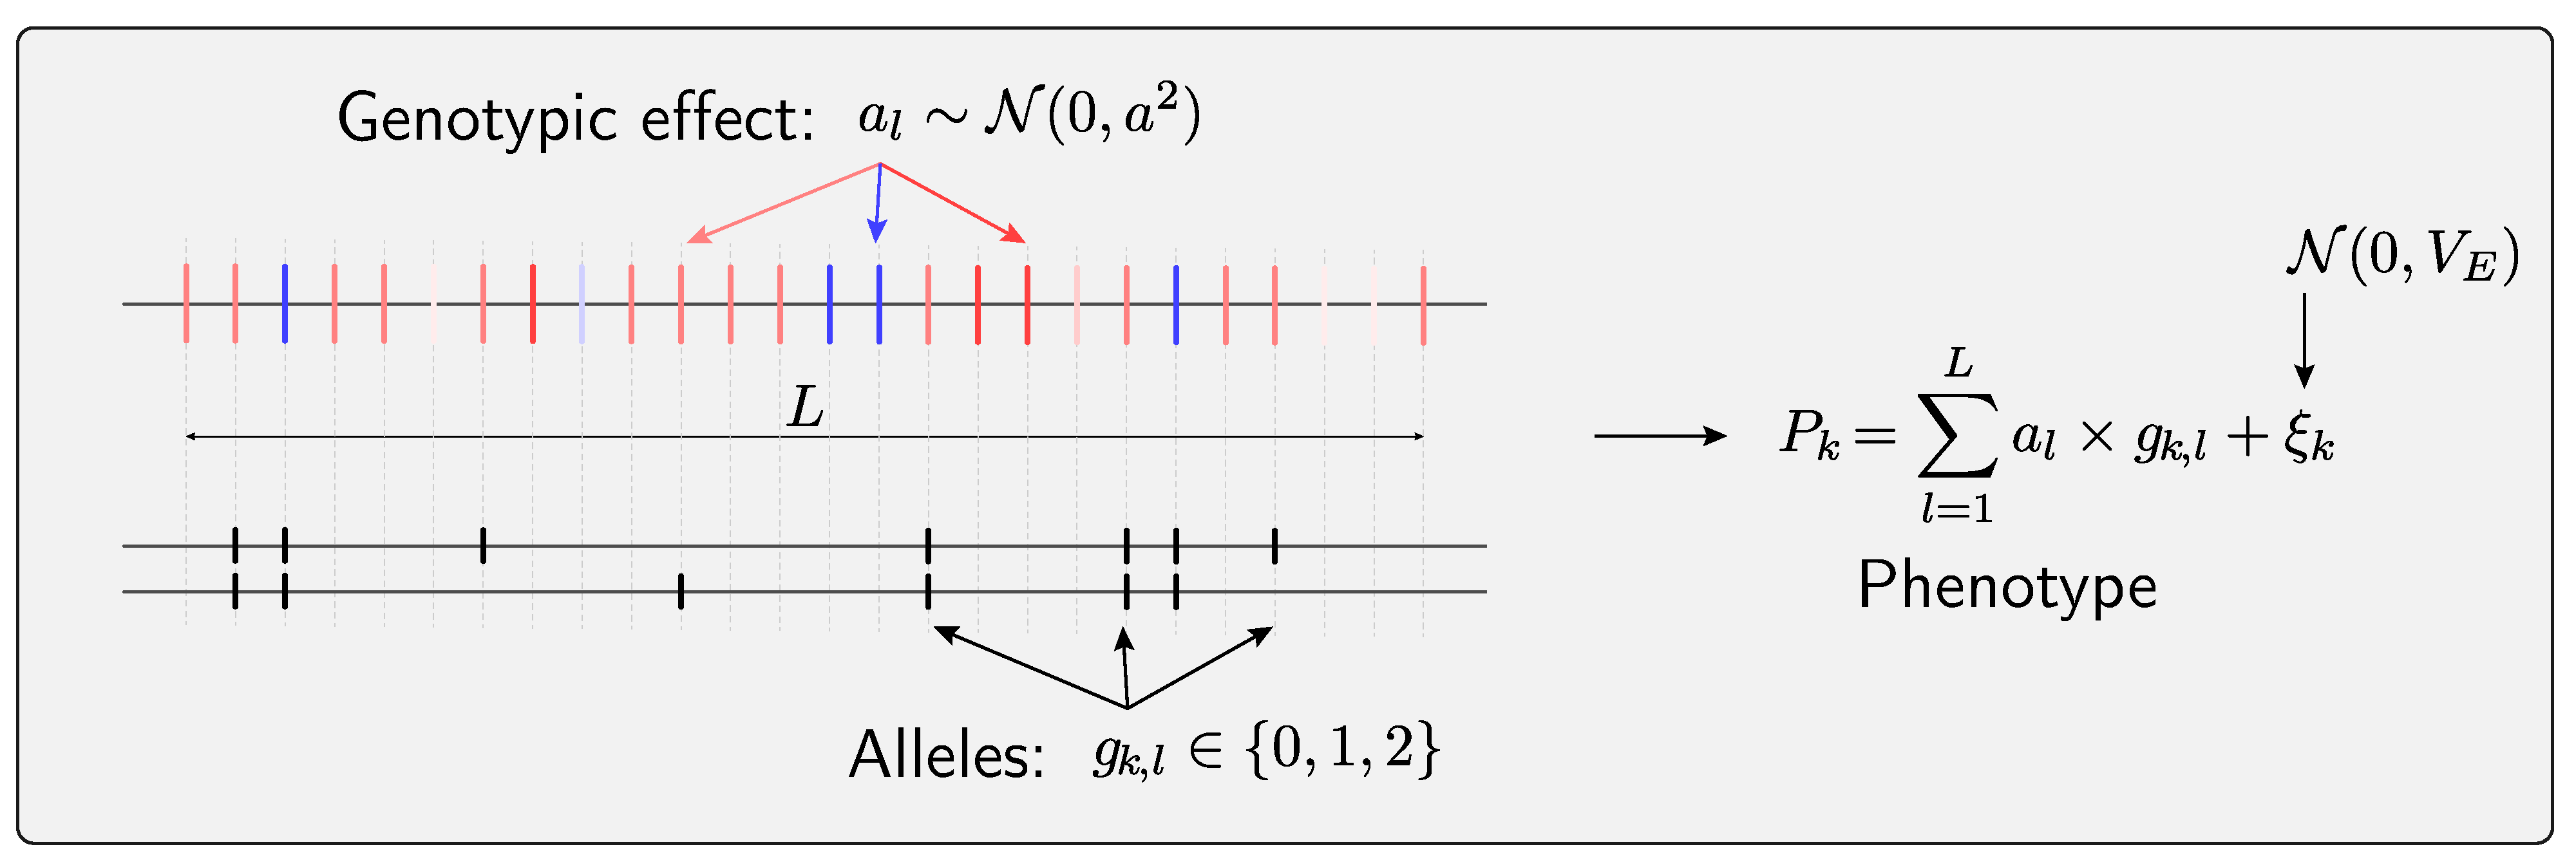
\includegraphics[width=0.6\textwidth, page=1] {figureS1}
    \label{fig:simulator-summary}
\end{center}

within-species, the mean ($\bar{G}$) and variance ($\VarGenetic$) of the genotype are:
\begin{equation}
    \bar{G} = \frac{1}{\Ne}\sum_{i=1}^{\Ne} G_i  \text{\quad and \quad} \VarGenetic = \frac{1}{\Ne}\sum_{i=1}^{\Ne}\left(G_i - \bar{G} \right)^2\label{eq:simu-genotype}
\end{equation}
The theoretical additive genetic variance ($\VarGenetic$) is a function of the number of loci ($\NbrLoci$) and the effect of a mutation ($a$) as:
\begin{equation}
    \VarGenetic = 4 \Ne \Multiply \MutationRatePheno \Multiply \NbrLoci \Multiply a^2 \label{eq:simu-var-genetic}
\end{equation}

The mean ($\bar{\Trait}$) and variance ($\VarPhenotype$) of the phenotype are:
\begin{equation}
    \bar{\Trait} = \frac{1}{\Ne}\sum_{i=1}^{\Ne} \Trait_i \text{\quad and \quad} \VarPhenotype = \frac{1}{\Ne}\sum_{i=1}^{\Ne}\left(\Trait_i - \bar{\Trait} \right)^2 \label{eq:simu-between}
\end{equation}

Heritability ($\Heritability$) is defined as:
\begin{equation}
    \Heritability = \frac{\VarGenetic}{\VarPhenotype} = \frac{\VarGenetic}{\VarGenetic + \VarEnv}\label{eq:simu-heritability}
\end{equation}
Altogether, effective population size ($\Ne$), the number of loci ($\NbrLoci$) and the effect of a mutation ($a$), we can compute the variance of the environment ($\VarEnv$) that is required to reach a given heritability ($\Heritability$) as:
\begin{equation}
    \VarEnv = \VarGenetic \Multiply \left( \frac{1}{\Heritability} - 1 \right) = 4 \Ne \Multiply \MutationRatePheno \Multiply \NbrLoci \Multiply a^2 \Multiply \left( \frac{1}{\Heritability} - 1 \right) \label{eq:simu-var-env}
\end{equation}

\newpage
\section{Bayesian estimate}\label{sec:bayesian-estimate}

\subsection{Multivariate Brownian process}\label{subsec:multivariate-brownian-process}
Here we generalize to $\Ntrait$ traits evolving along the phylogeny and are correlated between them.
Their variation along the phylogeny is modeled as a $\Ntrait$-dimensional Brownian process $\Brownian$ ($1 \times \Ntrait$) starting at the root and branching along the tree topology.
The rate of change of the Brownian process is determined by the positive semi-definite and symmetric covariance matrix between traits $\CovarianceMatrix$ ($\Ntrait \times \Ntrait$).
Along branch $j$ with length $d_{j}$, the Brownian process start at the ancestral node $\mathcal{A}(j)$ with value $\Brownian(\mathcal{A}(j))$, and ends at node $\mathcal{R}(j)$  with value $\Brownian(\mathcal{R}(j))$.
The independent contrast $\contrast_{j}$ defined as change in trait along the branch normalized by $\sqrt {d_{j}}$ is a multivariate Gaussian:
\begin{equation}
    \label{eq:DistribBrownian}
    \contrast_{j} = \frac{\Brownian (\mathcal{R}(j)) - \Brownian (\mathcal{A}(j)) }{\sqrt {d_{j}}} \sim \mathcal{N}\left(\VecZero, \CovarianceMatrix \right).
\end{equation}

\subsection{Sampling the covariance matrix}\label{subsec:sampling-the-covariance-matrix}
From the independent contrast at each branch of the tree ($\contrast_{j}$), we can define the $\Ntrait \times \Ntrait$ scatter matrix, $\Scattermatrix$, as:
\begin{equation}
    \Scattermatrix = \sum\limits_{j=1}^{\Nbranch} \contrast_{j} \MultiplyMatrix \left[\contrast_{j}\right]\tr\label{eq:bayes-scatter},
\end{equation}
where $\Nbranch$ is the number of branches in the tree and $\NbrTaxa$ the number of taxa.

The {prior} on the covariance matrix is an inverse Wishart distribution, with $\Ntrait + 1$ degrees of freedom:
\begin{equation}
    \label{eq:Distribcovariance}
    \CovarianceMatrix \sim \text{Wishart}^{-1} (\Identitymatrix, \Ntrait + 1).
\end{equation}

By Bayes theorem, the {posterior} on $\CovarianceMatrix$, conditional on a particular realization of $\Brownian$ (and thus of $\contrast$) is an invert Wishart distribution, of parameter $\Identitymatrix + \Scattermatrix$ and with $\WishartPostDf$ degrees of freedom.
\begin{equation}
    \CovarianceMatrix \sim \text{Wishart}^{-1}\left( \Identitymatrix + \Scattermatrix, \WishartPostDf\right)\label{eq:bayes-posterior}
\end{equation}
This invert Wishart distribution can be obtained by sampling $\WishartPostDf$ independent and identically distributed multivariate normal random variables $\Multivariate_{k}$ defined by
\begin{equation}
    \Multivariate_{k} \sim \mathcal{N} \left( \VecZero, \left[ \Identitymatrix + \Scattermatrix\right]^{-1} \right).\label{eq:bayes-multivariate}
\end{equation}
And from these multivariate samples, $\CovarianceMatrix$ is Gibbs sampled as:
\begin{equation}
    \CovarianceMatrix = \left( \sum\limits_{k=1}^{\WishartPostDf} \Multivariate_{k} \MultiplyMatrix  \left[\Multivariate_{k} \right] \tr \right)\inv \label{eq:bayes-gibbs}
\end{equation}

\newpage
\section{Bayesian and Maximum-likelihood implementation}\label{sec:implementation}

Implementation is included within the \textit{BayesCode} software, available at \censor{\url{https://github.com/ThibaultLatrille/bayescode}}.

\subsection{Data formatting}\label{subsec:data-formatting}

Running the analysis on your dataset and compute posterior probabilities requires three files:
\begin{enumerate}
    \item A phylogenetic tree in newick format, with branch lengths in number of substitutions per site (neutral markers)\DIFdelbegin \DIFdel{.
    }\DIFdelend \DIFaddbegin \DIFadd{, from which the values of nucleotide divergence ($d$) used in denominator of eq.~\ref{eq:estimated-rate-phy} are used.
    }\DIFaddend \item A file containing the mean trait values for each species.
    \item A file containing the variation within-species for each trait and the genetic variation within-species (neutral markers).
\end{enumerate}

\subsubsection{Phylogenetic tree}
\DIFdelbegin %DIFDELCMD < \label{subsubsec:phylogenetic-tree}
%DIFDELCMD < %%%
\DIFdelend 

The phylogenetic tree must be in newick format, with branch lengths in substitutions per site (neutral markers).

\subsubsection{Mean trait for each species}
\DIFdelbegin %DIFDELCMD < \label{subsubsec:mean-trait-for-each-species}
%DIFDELCMD < %%%
\DIFdelend 

The file containing mean trait values for each species must be in a tab-delimited file with the following format:
\begin{center}
    \begin{adjustbox}{width = 0.35\textwidth}
        \begin{tabular}{|l|c|c|}
            \hline
            TaxonName            & Body\_mass & Brain\_mass \\
            \hline
            Panthera\_tigris     & 12.26      & 5.676       \\
            Pithecia\_pithecia   & 7.256      & 3.436       \\
            Colobus\_angolensis  & 9.176      & 4.284       \\
            Saimiri\_boliviensis & 6.845      & 3.279       \\
            $\vdots$             & $\vdots$   & $\vdots$    \\
            \hline
        \end{tabular}\label{tab:trait-mean}
    \end{adjustbox}
\end{center}

The columns are:
\begin{itemize}
    \item \emph{TaxonName}: the name of the taxon matching the name in the alignment and the tree.
    \item As many columns as traits, without spaces or special characters in the trait.
    \item The values can be \texttt{NaN} to indicate that the trait is not available for that taxon.
\end{itemize}

\newpage
\subsubsection{Trait variation for each species}
\DIFdelbegin %DIFDELCMD < \label{subsubsec:trait-variation-for-each-species}
%DIFDELCMD < %%%
\DIFdelend 

The file containing trait variation for each species must be in a tab-delimited file with the following format:
\begin{center}
    \begin{adjustbox}{width = 1.0\textwidth}
        \begin{tabular}{|l|c|c|c|c|c|c|}
            \hline
            TaxonName            & Nucleotide\_diversity & Body\_mass\_variance & Body\_mass\_heritability & Brain\_mass\_variance & Brain\_mass\_heritability \\
            \hline
            Pithecia\_pithecia   & 0.0016                & 0.22871              & 0.2                      & 0.00737               & 0.2                       \\
            Colobus\_angolensis  & 0.0017                & 0.00393              & 0.2                      & 0.00416               & 0.2                       \\
            Saimiri\_boliviensis & 0.0013                & 0.00022              & 0.2                      & 0.00045               & 0.2                       \\
            Pygathrix\_nemaeus   & 0.0016                & 0.00347              & 0.2                      & 0.00097               & 0.2                       \\
            $\vdots$             & $\vdots$              & $\vdots$             & $\vdots$                 & $\vdots$              & $\vdots$                  \\
            \hline
        \end{tabular}
        \label{tab:trait-variance}
    \end{adjustbox}
\end{center}

\begin{itemize}
    \item \emph{TaxonName}: the name of the taxon matching the name in the alignment and the tree.
    \item \emph{Nucleotide\_diversity}: the nucleotide diversity within-species (neutral markers), cannot be \texttt{NaN}.
    \item As many columns as traits, without spaces or special characters in the trait.
    \item \emph{TraitName\_variance}: the phenotypic variance of the trait within-species, can be \texttt{NaN} to indicate that the trait variance is not available for that taxon.
    \item \emph{TraitName\_heritability} (optional): the heritability of the trait within-species, between 0 and 1, cannot be \texttt{NaN}.
    \item The columns with the suffix \texttt{\_variance} and \texttt{\_heritability} are repeated for each trait.
    \item \emph{TraitName\_heritability\_lower} (optional): the lower bound of the heritability of the trait within-species, between 0 and 1, cannot be \texttt{NaN}.
    \item \emph{TraitName\_heritability\_upper} (optional): the upper bound of the heritability of the trait within-species, between 0 and 1, cannot be \texttt{NaN}.
    \item If the columns with the suffix \texttt{\_heritability\_lower} and \texttt{\_heritability\_upper} are present, the heritability is randomly drawn from a uniform distribution between the lower and upper bounds.
    \item If the columns with the suffix \texttt{\_heritability} is present, it is taken as is.
    \item If the additive genetic variance (instead of phenotypic variance) is available for a trait, the heritability can be omitted and will automatically be set to 1.0.
\end{itemize}

\newpage
\subsection{Bayesian estimation}\label{subsec:running-nodetraitsand-readnodetraits}

The executable \texttt{nodetraits} from \textit{BayesCode} is used to run the Bayesian estimation of the model, and the executable \texttt{readnodetraits} is used to read the results.

Assuming that the file \texttt{data/body\_size/mammals.male.tsv} contains the mean trait values for each species, the file \texttt{data/body\_size/mammals.male.var\_trait.tsv} contains the variation within-species for each trait and the genetic variation within-species (neutral markers), and the file \texttt{data/body\_size/mammals.male.tree} contains the phylogenetic tree, the following commands are used to run the model and read the results.

\subsubsection{Running the model}
\DIFdelbegin %DIFDELCMD < \label{subsubsec:running-nodetraits}
%DIFDELCMD < %%%
\DIFdelend \texttt{nodetraits} is run with the following command:
\begin{lstlisting}[language = sh,label={lst:nodetraits-run}]
nodetraits  --until 2000
            --tree data/body_size/mammals.male.tree
            --traitsfile data/body_size/mammals.male.tsv
            run_mammals_male
\end{lstlisting}

\subsubsection{Reading the results}
\DIFdelbegin %DIFDELCMD < \label{subsubsec:reading-the-results}
%DIFDELCMD < %%%
\DIFdelend Once the model has run, the chain \texttt{run\_mammals\_male} is used to compute the posterior distribution of the ratio of between-species variation over within-species variation with \texttt{readnodetraits}:
\begin{lstlisting}[language = sh,label={lst:readnodetraits-rho}]
readnodetraits --burnin 1000
               --var_within data/body_size/mammals.male.var_trait.tsv
               --output results_mammals_male.tsv
               run_mammals_male
\end{lstlisting}
The file \texttt{data\_empirical/chain\_name.ratio.tsv} then contains the posterior mean of the ratio of between-species variation over within-species variation, the 95\% and 99\% credible interval, and the posterior probability that the ratio is greater than 1.

\subsection{Maximum likelihood estimation}\label{subsec:maximum-likelihood-estimation}

To obtain the ratio (without the posterior credible interval and probability) using maximum likelihood computation, the following python script can be used:
\begin{lstlisting}[language = sh, label={lst:neutrality_index}]
python3 utils/neutrality_index.py --tree data/body_size/mammals.male.tree
                                  --traitsfile data/body_size/mammals.male.tsv
                                  --var_within data/body_size/mammals.male.var_trait.tsv
                                  --output results_ML_mammals_male.tsv
\end{lstlisting}
\DIFaddbegin 

\newpage
\section{\DIFadd{Saturation of phenotypic divergence}}\label{sec:supp-distance}

\DIFadd{The phenotype is encoded by a genetic architecture and is thus ultimately bounded.
At the macro-evolutionary scale, phenotypic divergence should plateau at some point, ultimately resulting in a $\RateBetween$.
}

\begin{center}
    \captionof{figure}{Saturation of phenotypic divergence.}
    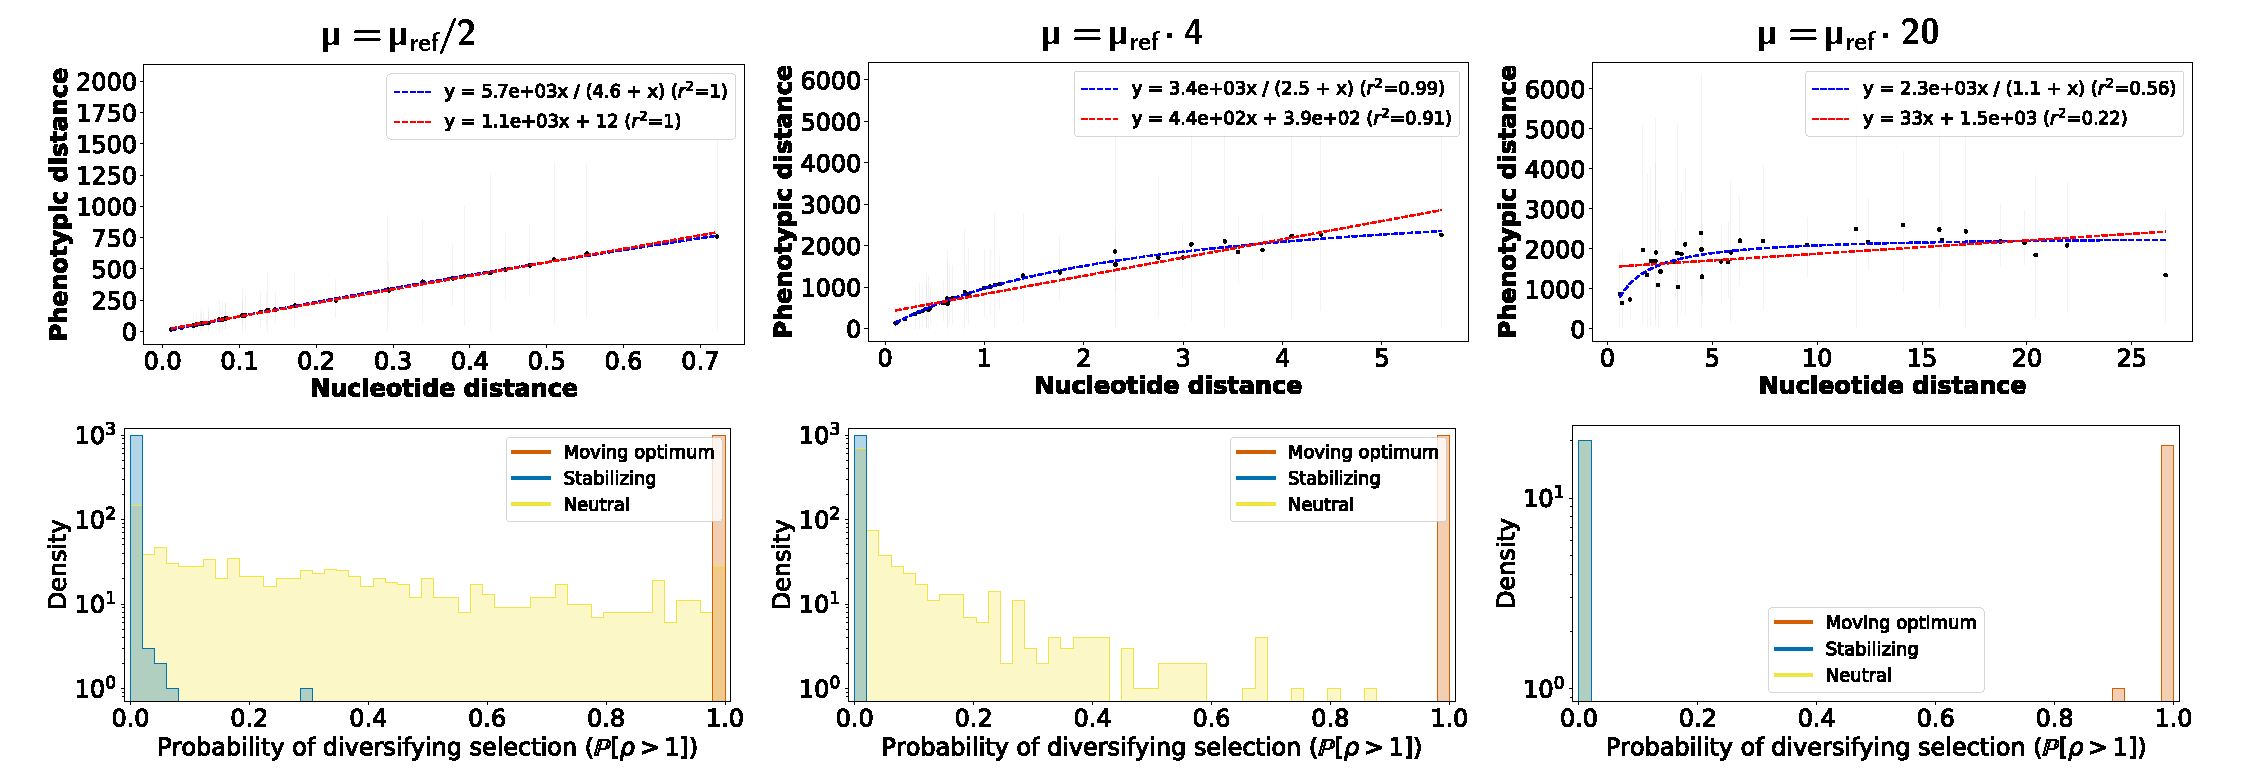
\includegraphics[width=1.0\textwidth, page=1] {figureS2}
    \label{fig:supp-distance}
\end{center}
\begin{itemize}
    \item \DIFadd{Left column: $1,000$ simulations with low divergence between species (half that of mammals).
    }\item \DIFadd{Middle column: $1,000$ simulations with high divergence between species (4 times that of mammals).
    }\item \DIFadd{Right column: $200$ simulations with very high divergence between species (20 times that of mammals).
    }\item \DIFadd{Top row: Simulation of neutral trait, phenotypic divergence between species as a function of the nucleotide divergence. Phenotypic divergence is computed between two species as the covariance between the trait ($\VarPhy$), and the nucleotide divergence is computed as the number of substitutions per site shared between the two species ($d$). Each point is a pair of species, and the bounds of the intervals in grey are the 2.5\% and 97.5\% quantiles across the replicates. The blue line is the linear regression and the red line is the saturation model ($y = \alpha \Multiply x / (\beta + x)$).
    }\item \DIFadd{Bottom row: Traits simulated under stabilizing selection (blue), under a neutral evolution (yellow), and under a moving optimum (red). Histogram of probabilities of $\EstNI$ being greater than $1$.
}\end{itemize}
\DIFadd{Under a model of neutral trait evolution, when mutation rate increases, or equivalently the divergence between species increases, the phenotypic divergence between species saturates faster than the nucleotide divergence.
This saturation effect can result in a spurious signal of stabilizing selection ($\EstNI < 1$) for deeper phylogeny when the trait is evolving neutrally.
 }\DIFaddend\end{document}
%TC:endignore